\chapter{Area exploration}\label{chap:area_exploration}
different time exploration
imu to switch off
time following


jksdbkvbdsjg\\
 jksdbkvbdsjg\\
jksdbkvbdsjg\\
 jksdbkvbdsjg\\
jksdbkvbdsjg\\
 jksdbkvbdsjg\\
jksdbkvbdsjg\\
 jksdbkvbdsjg\\
jksdbkvbdsjg\\
 jksdbkvbdsjg\\
jksdbkvbdsjg\\
 jksdbkvbdsjg\\
jksdbkvbdsjg\\
 %TODO
\begin{figure}[!htbp]
    \centering
    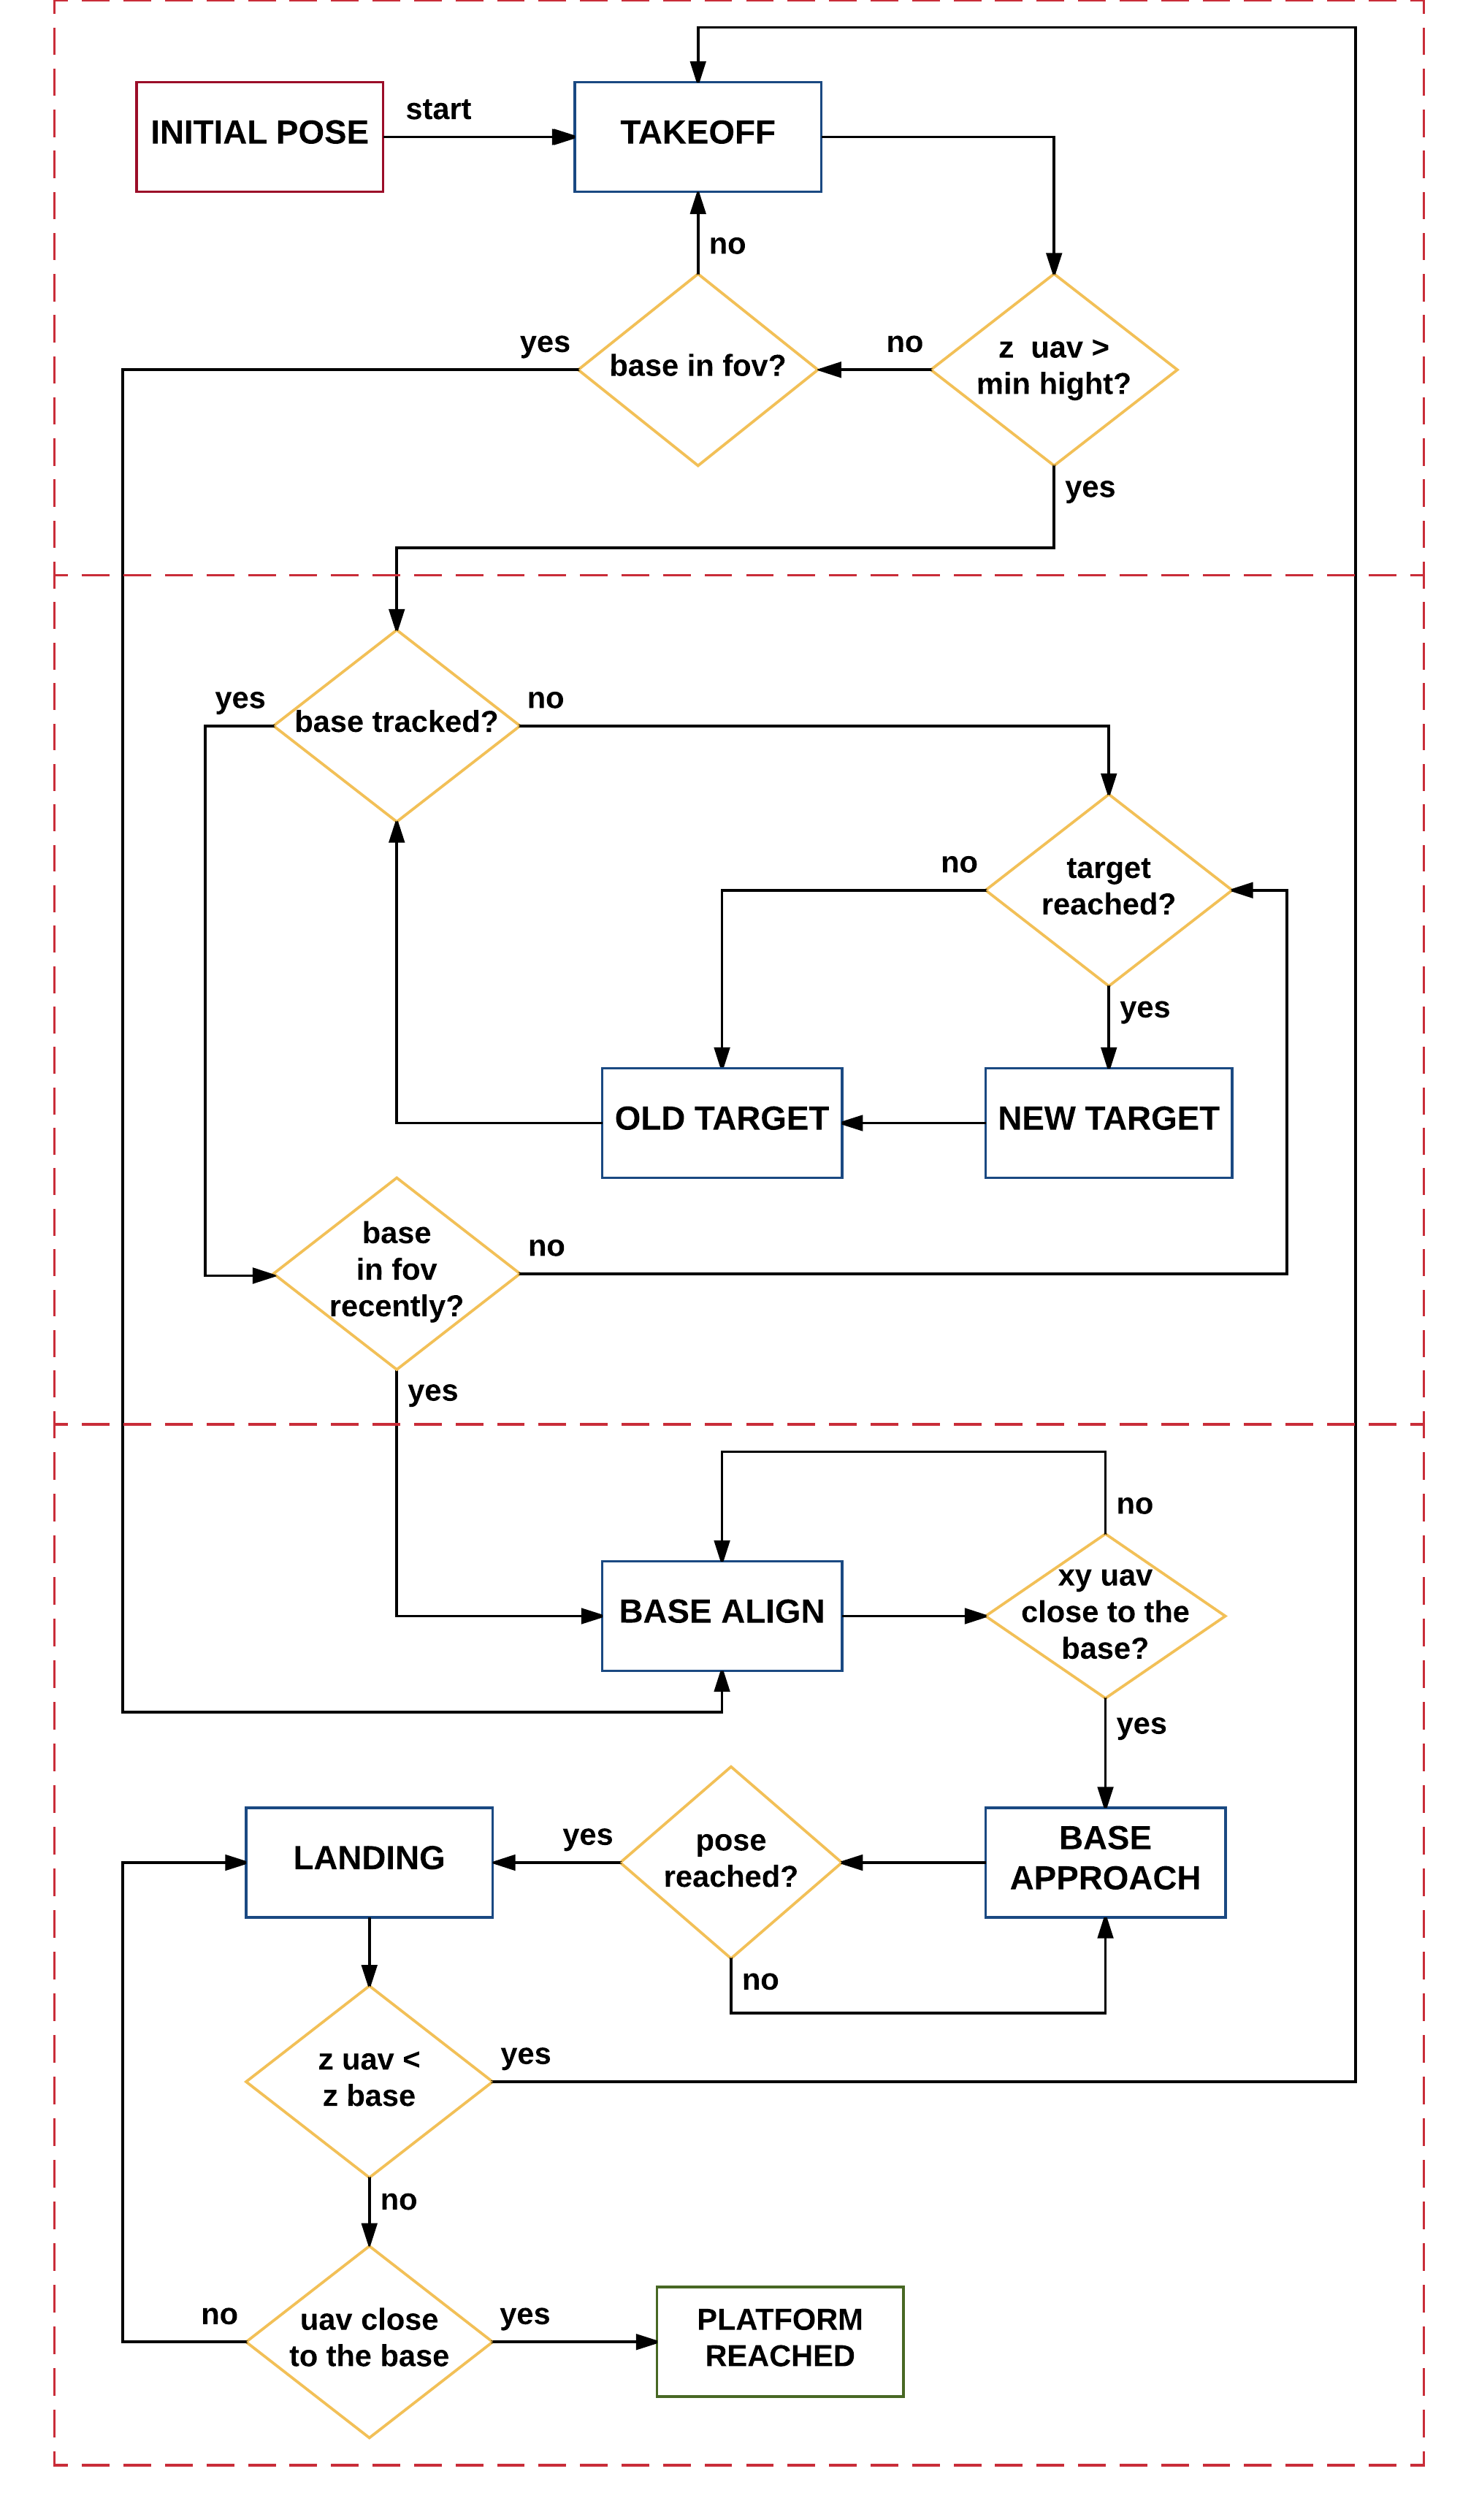
\includegraphics[width=0.9\textwidth]{img/area_exploration_state_machine.png}
    \caption{Area Exploration}
    \label{fig:area_exploration_state_machine}
\end{figure}

\section{Phases}
\subsection{First phase - Searching for the base}
In this phase the quadrotor starts from a given position and has to find the moving car.
Given the rectangle in which the platform can move the UAV follows a list of way-points in order to span the whole area at high altitude. In this way the downward camera can collect information from a large section of the space and the searching task can be performed faster.\\

\subsubsection{Understand type of movement}
From the challenge description \ref{fig:arenachallenge} we know that the car is moving in a shape composed by straight lines and circumference sectors. We need to understand in which part is the platform at a given time: this information is important in order to calculate properly where the platform will be in $t$ seconds and because we want to proceed with the following phases, and finally perform the landing maneuver, when the platform is going straight.\\
To understand the trajectory of the moving base we collect all the estimated positions of the base, and we perform a linear regression on the last $n$ estimations: the platform is moving in a straight line if the linear regression is a good approximation of the data trends otherwise it driving in a curve.\\


We have a series of $n$ points, each of these is consider as a pair of coordinates $(x_i,y_i)$, and we are searching for he best-fit line that can describe the data as a linear function:  $$y = mx + q$$ 
(we perform the following analysis considering before the coordinates $y_i$ as dependent variables, then $x_i$, and we are peaking the best of this two fits). \\
We want find the best best parameters $m$ and $q$, and to do so we need to have some measure of quality to optimize. Unless all our $n$ points are already in a perfect line (trivial solution), there will be an error between the value predicted by the line, and the observed dependent variable:
$$e_i = y_i - (mx_i + q)$$
These differences are called residuals and what we want is to find a line that minimizes: 
$$\sum_{i=1}^{n}{e_i^2}$$
The model we find is the Least Squares Fit of the data. \\ %TODO cite
We define also the cumulative residual as: $$e_{tot} = \sqrt{\sum_{i=1}^{n}{e_i^2}}$$
The parameters $m$ and $q$ of the model, are found where $e_{tot}^2$ is minimized:
\begin{align}
\begin{split}
\frac{e_{tot}^2}{\partial m} = 0\\
\frac{e_{tot}^2}{\partial q} = 0
\end{split}
\label{eq:mandq1}
\end{align}
It is easy to demonstrate that the solution of \ref{eq:mandq1} is:
\begin{align}
\begin{split}
m &= \frac{n\sum_{i=1}^{n}{x_iy_i} - \sum_{i=1}^{n}{x_i}\sum_{i=1}^{n}{y_i}}{n\sum_{i=1}^{n}{x_i^2} -( \sum_{i=1}^{n}{x_i})^2} \\
q &= \frac{ \sum_{i=1}^{n}{y_i}}{n} - m\frac{ \sum_{i=1}^{n}{x_i}}{n}\\
\end{split}
\label{eq:mandq}
\end{align}

The platform is moving in the straight line if the cumulative residual $e_{tot}$ is below a threshold $th_{line}$, while if the error is above $th_{curve}$ the base is following the circumference.\\

To have a good interpretation of the data it is important to decide the three parameters $n$, $t_{line}$, $t_{curve}$ correctly.\\
\begin{itemize}
\item The first parameter $n$ is the number of samples to consider when we perform the linear regression. We chose it in order to consider poses that are along a curve with length 
\begin{align}
l_{curve} = \frac{r_{8}\pi}{4} \label{eq:lengthcurve} 
\end{align}
We know the forward constant velocity of the car $v_{tan}$, so we can calculate the time in which the platform is performing the curve 
\begin{align}
t_{curve} = \frac{l_{curve}}{v_{tan}} \label{eq:timecurve} 
\end{align}

When we receive a pose at time $t_i$ we store it and we perform the linear regression with all the data stored from $[t_i-t_{curve},t_i]$.
\item The threshold parameters are calculating considering that each measure is corrupted by an additive Gaussian noise with 0 mean and $\sigma_e^2$ variance: $$\tilde{y_i} = \mathcal{N}(y_i,\sigma_e^2) $$
When we perform the linear regression on the measured data, the average residual square is 
\begin{align}
\begin{split}
<\tilde{e_i}^2> &= \\
<(\tilde{y_i} - (mx_i + q))^2>  &= \\
<\tilde{y_i}^2 - 2\tilde{y_i}(mx_i + q) + (mx_i + q)^2> &= \\
<\tilde{y_i}^2> - 2<\tilde{y_i}>(mx_i + q) + (mx_i + q)^2 &= \\
\sigma_e^2 + y_i^2  - 2y_i(mx_i + q) + (mx_i + q)^2 &=  \\
\sigma_e^2 + e_i^2 
\end{split}
\end{align}

\begin{itemize}
\item when we perform the linear regression on linear data the theoretical residual is 
$$e_i = 0$$
And the average residual squares on the measured data $$<\tilde{e_i}^2>  = \sigma_e^2$$. \\
The parameter $th_{line}$ is then:
\begin{align}
\begin{split}
th_{line} = \sqrt{\sum_{i=1}^{n}{\tilde{e_i}^2}} = \sqrt{\sum_{i=1}^{n}{\sigma_e^2}} = \sigma_e\sqrt{n}
\end{split}
\end{align}
\item when we perform the linear regression on data along a circumference arch with radius $\rho$ and angles $\theta_i \in [\theta_1,\theta_2]$ the theoretical data are distributed as:
$$(\rho\cos{\theta_i},\rho\sin{\theta_i})$$ 
so the theoretical residual is:
$$e_i = \rho\sin{\theta_i} - (m\rho\cos{\theta_i} + q)$$
To find $m$ and $q$ we use equation \ref{eq:mandq}, but we want a general approximation of these values. To do so, we have  to consider all the sums in the equations as integrals, using the relation \ref{eq:integralsandsums}
\begin{align}
\begin{split}
\lim_{n \to \infty} { \frac{b-a}{n} \sum_{i=0}^{n}{f(x_i)}} =   \int_a^b{f(x )\mathrm  {d}x} \\
 \sum_{i=0}^{n}{f(x_i)} \simeq \frac{n}{b-a} \int_a^b{f(x )\mathrm  {d}x}
\end{split}
\label{eq:integralsandsums}
\end{align} 
So now if we calculate this approximation for our values we have:
\begin{align}
\begin{split}
\sum_{i=1}^{n}{x_iy_i} &= \sum_{i=1}^{n}{\rho^2\cos{\theta_i}\sin{\theta_i}} \\
& \simeq  \frac{n}{\theta_2 - \theta_1}  \rho^2 \int_{\theta_1}^{\theta_2}{\cos{x}\sin{x} \mathrm  {d}x} =  \frac{n}{\theta_2 - \theta_1}  \frac{ \rho^2}{2} \Big[-\cos^2{x} \Big]_{\theta_2}^{\theta_2} \\
 \sum_{i=1}^{n}{x_i} &= \sum_{i=1}^{n}{\rho\cos{\theta_i}} \\
&\simeq  \frac{n}{\theta_2 - \theta_1}  \rho \int_{\theta_1}^{\theta_2}{\cos{x}\mathrm  {d}x} = \frac{n}{\theta_2 - \theta_1}  \rho \Big[\sin{x} \Big]_{\theta_2}^{\theta_2}\\
 \sum_{i=1}^{n}{y_i} &= \sum_{i=1}^{n}{\rho\sin{\theta_i}} \\
& \simeq  \frac{n}{\theta_2 - \theta_1}  \rho \int_{\theta_1}^{\theta_2}{\sin{x}\mathrm  {d}x} = \frac{n}{\theta_2 - \theta_1}  \rho \Big[-\cos{x} \Big]_{\theta_2}^{\theta_2}\\
 \sum_{i=1}^{n}{x_i^2} &= \sum_{i=1}^{n}{\rho^2\cos^2{\theta_i}} \\
& \simeq  \frac{n}{\theta_2 - \theta_1}  \rho^2 \int_{\theta_1}^{\theta_2}{\cos^2{x}\mathrm  {d}x} =  \frac{n}{\theta_2 - \theta_1}  \frac{ \rho^2}{2} \Big[ x+\cos{x} \sin{x}\Big]_{\theta_2}^{\theta_2}\\
\end{split}
\label{eq:mandqintegralsoncircum}
\end{align}
In our case we consider pieces of curve with length $l_{curve}$ \ref{eq:lengthcurve}, that corresponds to a circumference arch with:
\begin{align}
\rho = r_{8}  \ \ \ \ \ \ \ \ \ \ \ \ \ 
\theta_i \in \Big[0,\frac{\pi}{4}\Big]
\label{eq:valuessircum}
\end{align}

We can now calculate the approximate values of $m$ and $q$ using \ref{eq:mandq} \ref{eq:mandqintegralsoncircum} \ref{eq:valuessircum}:

\begin{align}
\begin{split}
m &= \frac{nr_{8}^2\frac{n}{\pi} - r_{8}\frac{n2\sqrt{2}}{\pi} r_{8}\frac{n2(2-\sqrt{2})}{\pi} }{n\frac{nr_{8}^2(2+\pi)}{2\pi} -(r_{8}\frac{n2\sqrt{2}}{\pi})^2} = \frac{2\pi - 16\sqrt{2} + 16}{\pi^2 + 2\pi - 16}  \\
q &= \frac{ r_{8}\frac{n2(2-\sqrt{2})}{\pi} }{n} - m\frac{ r_{8}\frac{n2\sqrt{2}}{\pi}}{n} = r_{8} \frac{4-2\sqrt{2}(m+1)}{\pi} = r_{8}\bar{q} \\
\end{split}
\label{eq:mandqcirum}
\end{align}
Now we can calculate the theoretical average residual square, using again the approximations  \ref{eq:mandqintegralsoncircum}:
\begin{align*}
\begin{split}
<e_i^2> &= \frac{\sum_{i = 1}^{n}{\Big(r_{8}\sin{\theta_i} - (mr_{8}\cos{\theta_i} + q)\Big)^2}}{n}\\
&= \frac{\sum_{i = 1}^{n}{\Big(r_{8}^2\sin^2{\theta_i} - 2r_{8}\sin{\theta_i}(mr_{8}\cos{\theta_i} + q) + (mr_{8}\cos{\theta_i} + q)^2\Big)}}{n}\\
& = \frac{\sum_{i = 1}^{n} r_{8}^2 \xi }{n} = r_{8}^2 \xi \\
\xi &= \frac{\pi - 2 + m^2(\pi+2) + 2\pi\bar{q}^2 - 4m -8\bar{q}(2-\sqrt{2}) + 8m\bar{q}\sqrt{2}}{2\pi}
\end{split}
\end{align*} 
Finally we calculate $$<\tilde{e_i}^2>  = <e_i^2> + \sigma_e^2 = \rho^2 \xi  + \sigma_e^2 $$. \\
The parameter $th_{curve}$ is:
\begin{align}
\begin{split}
th_{curve} = \sqrt{\sum_{i=1}^{n}{\tilde{e_i}^2}} = \sqrt{\sum_{i=1}^{n}{\rho^2 \xi  + \sigma_e^2}} = \sqrt{n}(\sigma_e + \rho\sqrt{\xi})
\end{split}
\end{align}
\end{itemize}
\end{itemize}
The figure \ref{fig:error_regression} shows the typical evolution of the total residual during this first phase: the different phases of linear and circular movement can be detect in the graph. Furthermore the point of regime change can be seen both in figure \ref{fig:error_regression}  and in the map \ref{fig:error_regression_map} in which also all the estimate positions of the base are plotted.\\


\begin{figure}[!htbp]
    \centering
    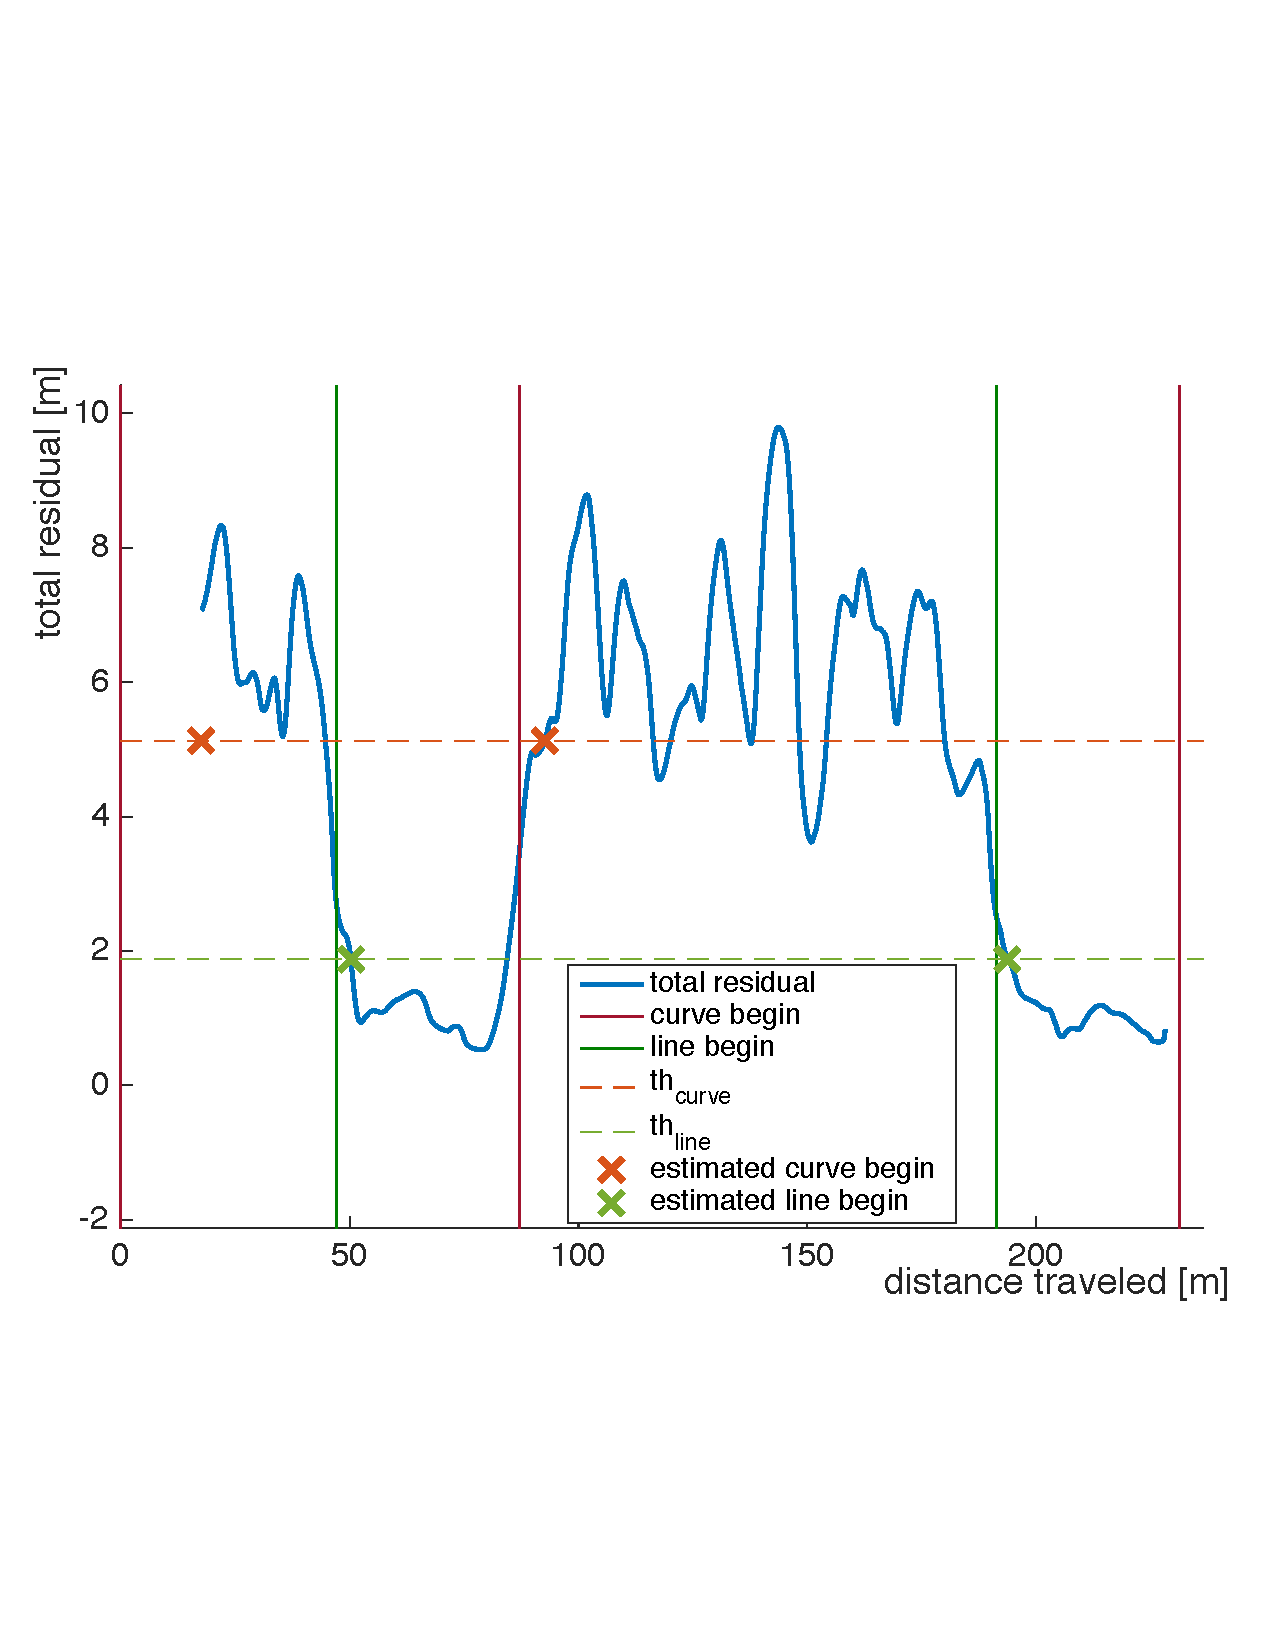
\includegraphics[width=1.0\textwidth]{img/following_platform_for_long_position_base_error.pdf}
    \caption{Evolution of the total residual during this first phase (in blue). The vertical lines are the real moments in which the car changes movement types: green a linear phase starts, red a circular phase begins. The horizontal lines are the thresholds for the detection of the two different regimes. The cross are the moment in which the algorithm understands the change.}
    \label{fig:error_regression}
\end{figure}

\begin{figure}[!htbp]
    \centering
    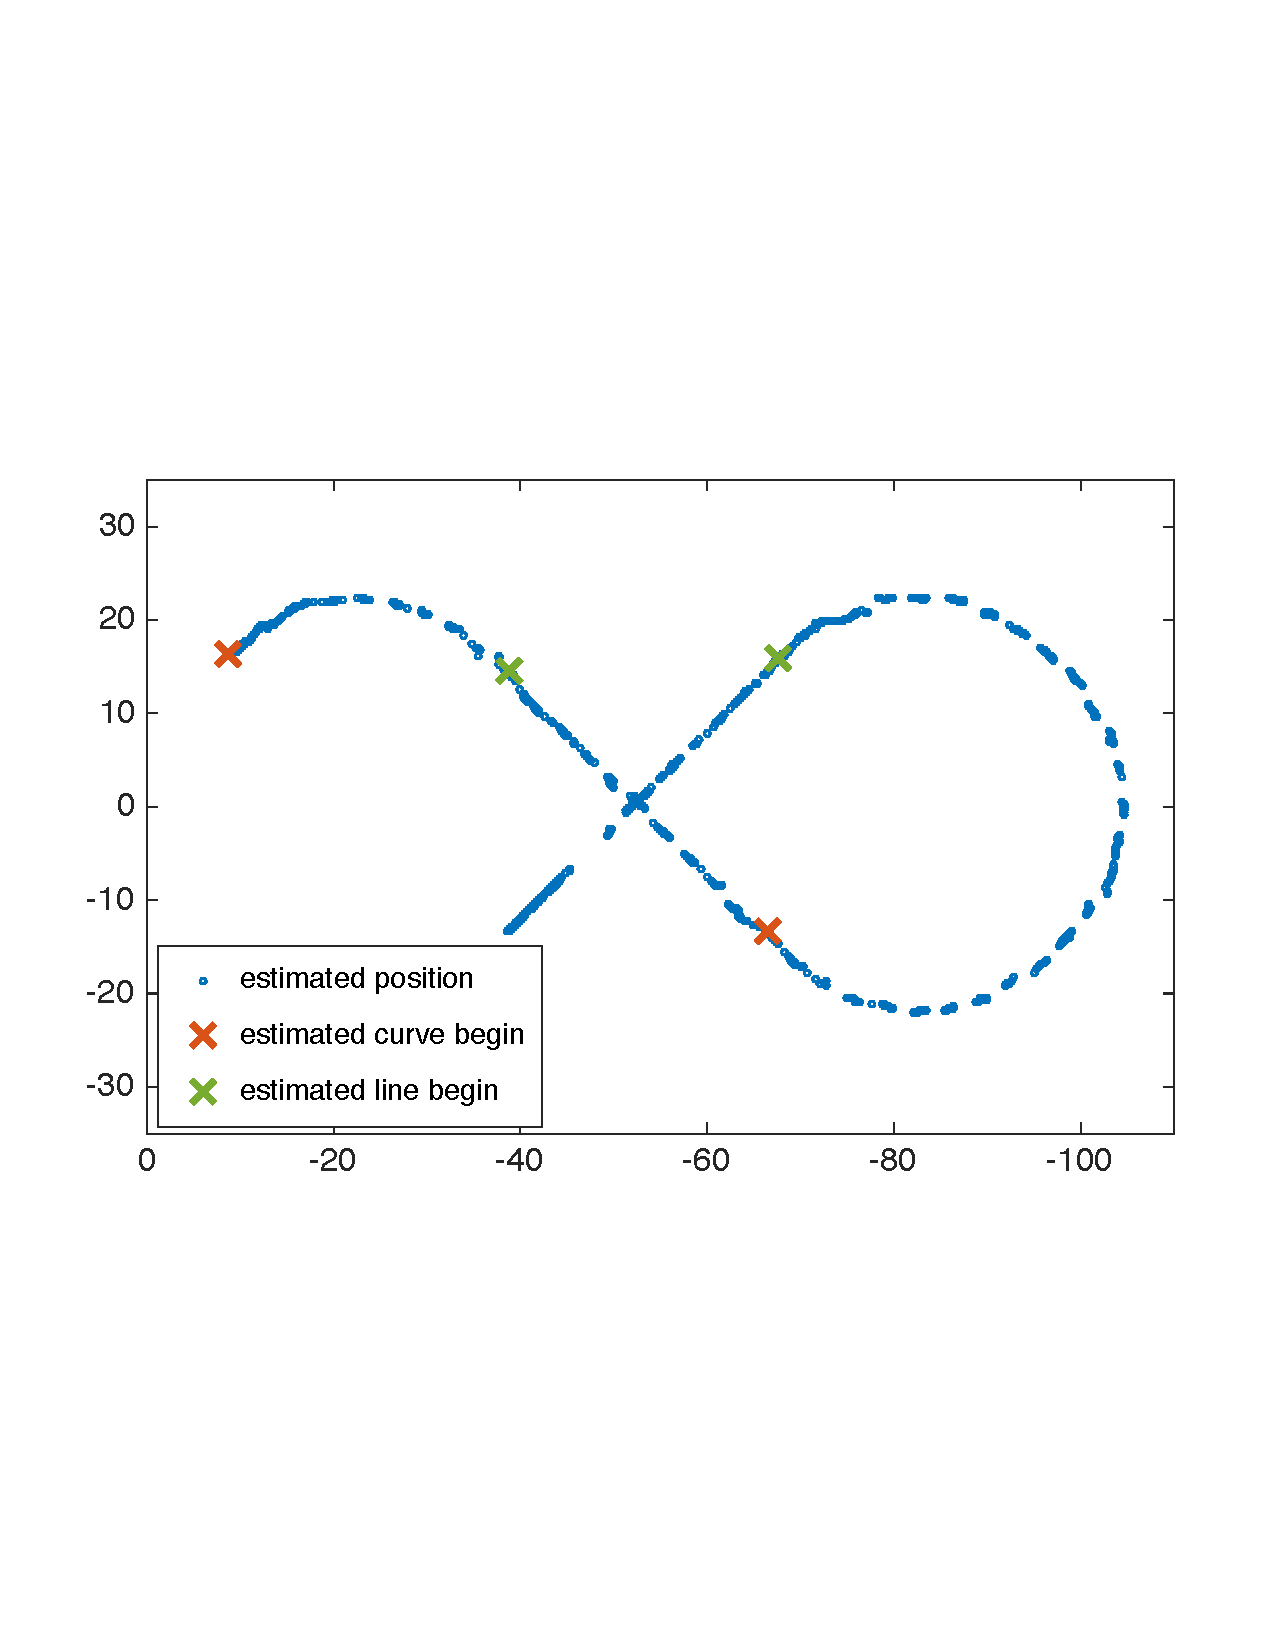
\includegraphics[width=0.7\textwidth]{img/following_platform_for_long_map_simple.pdf}
    \caption{Map of the estimated position of the car in blue. The cross are the moments in which the algorithm understands the change. Red crosses from line to curve. Green crosses from curve to line.}
    \label{fig:error_regression_map}
\end{figure}


\subsubsection{Calculate future position}
Now knowing the platform regime of movement at a specific time we can estimate correctly where it will be after $t_s$ seconds and proceed with the following phases when it starts a straight portion of the trajectory.\\
Thanks to the algorithm described before we can estimate that at the moment $t_0$ the car is at position $(x_0,y_0)$ with a direction angle of $\theta_0$ and forward velocity of $v_{tan}$, so at time $t_1 = t_0 + t_s$ seconds the car will be at position $(x_1,y_1)$ with an angle  $\theta_1$, and it has traveled  $v_{tan}t_s$.

\begin{itemize}
\item When no regime is found (at the begging) or when a line movement is detect, the predicted state is simply
\begin{align}
\begin{cases}
x_1 &= x_0 + v_{tan}t_s\cos{\theta_0}\\
y_1 &= y_0 + v_{tan}t_s\sin{\theta_0}\\
\theta_1 &= \theta_0
\end{cases}
\end{align}
\item When a movement in the circumference is detected we have to perform some calculations in order to find the final state of the platform.\\ 
First of all we use the relation 
$$l_{curve} = \rho|\beta_s|$$ 
To find the angle $\beta_s$ that the platform will span in $t_s$ seconds. In our case:
\begin{align}
\begin{split}
v_{tan}t_s &= r_8| \beta_{s}|\\
|\beta_{s}| &= \frac{v_{tan}t_s}{r_8}
\end{split}
 \label{eq:anglespanned}
\end{align}
The final angle will be:
 \begin{align}
 \theta_1 = \theta_0 + \beta_s
 \label{eq:anglefinal}
 \end{align}


The segment connecting $(x_0,y_0)$ and $(x_1,y_1)$ has \ref{fig:chord}:
\begin{itemize}
\item direction $\theta_{chord}$ found as bisection between 
 $\theta_0$ and $\theta_1$
 \begin{align}
 \theta_{chord} = \theta_0 + \frac{\theta_0 + \theta_1}{2} 
 \label{eq:anglechord}
 \end{align}
\item length $l_{chord}$, found with the chord theorem: %TODO
\begin{align}
 l_{chord} = 2r_8\sin{\frac{|\beta_s|}{2}}
  \label{eq:lengthchord}
 \end{align}
\end{itemize}
\begin{figure}[!htbp]
    \centering
    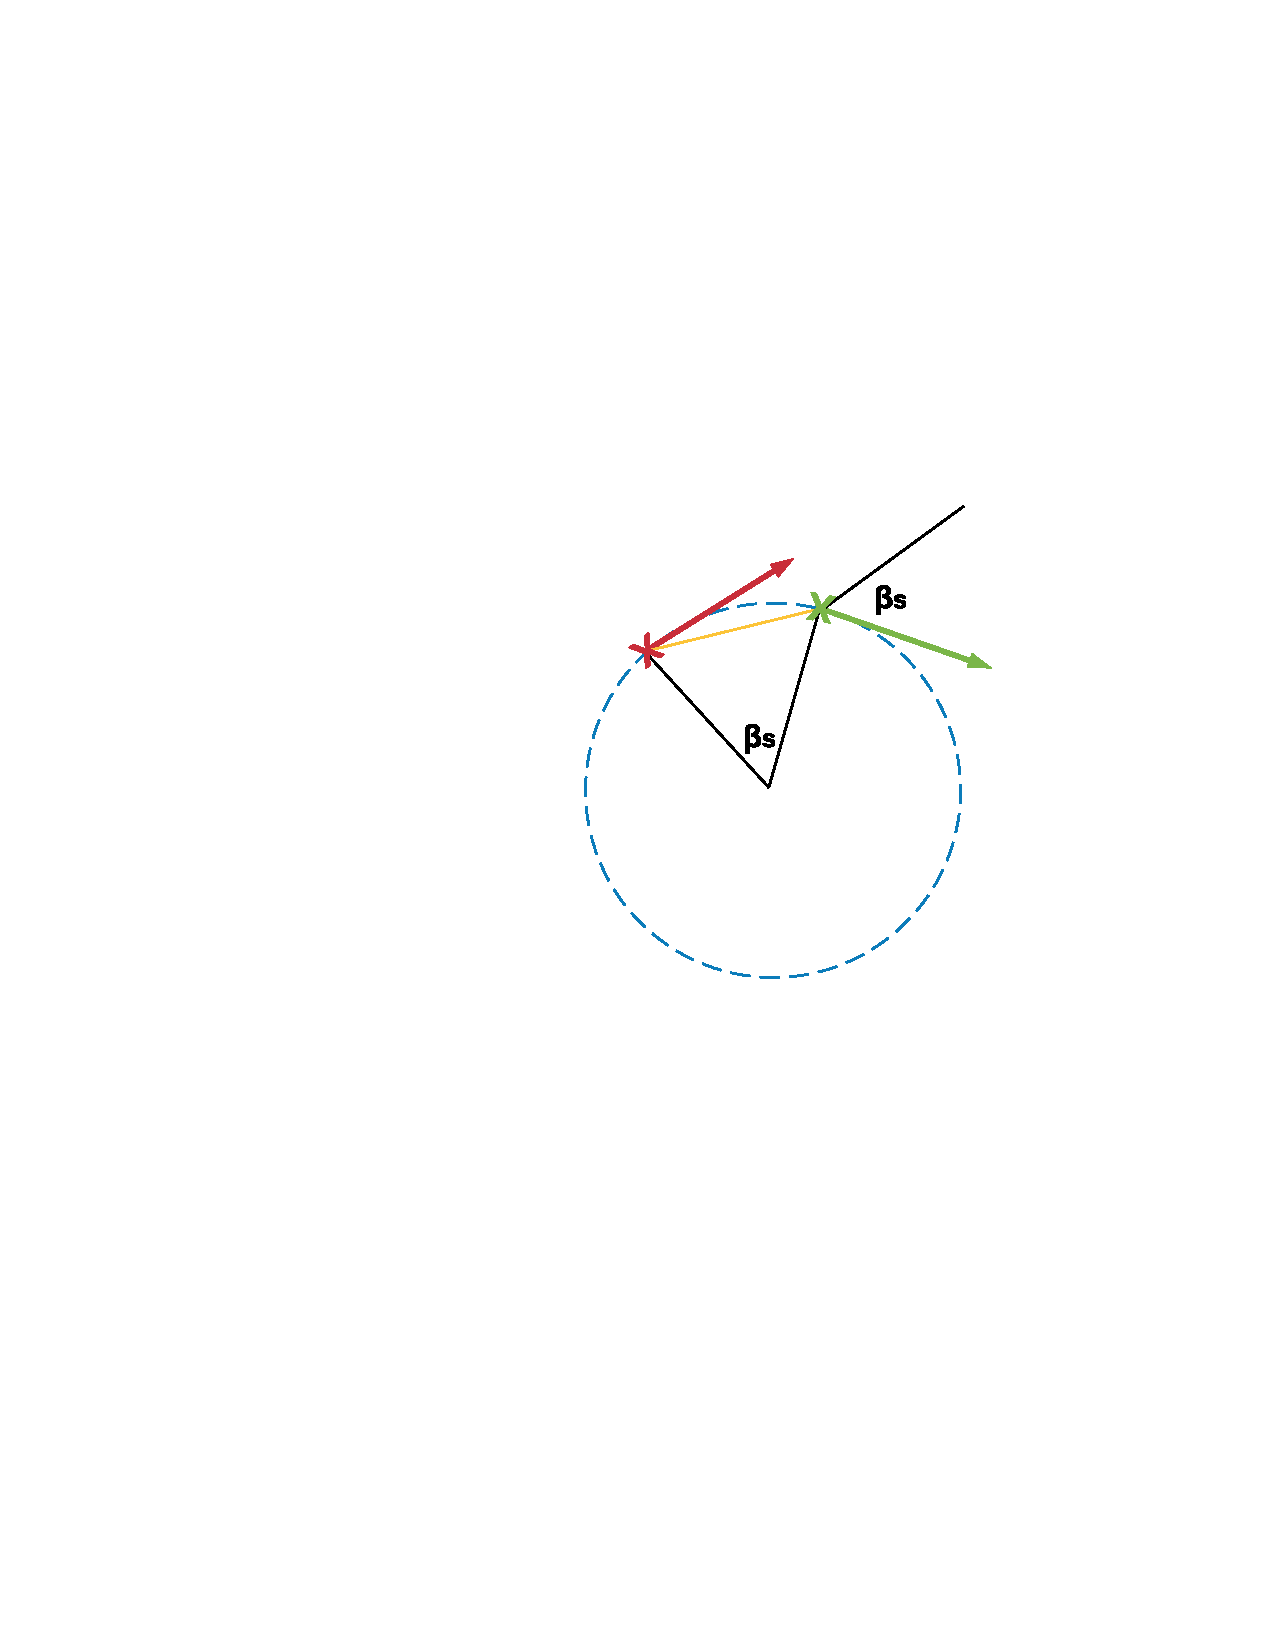
\includegraphics[width=0.35\textwidth]{img/chord.pdf}
    \caption{In red position of initial state at time $t_0$. In green final estimate state at time $t_1$. In yellow the chord between the two states with length $l_{chord}$ and orientation $\theta_{chord}$.}
    \label{fig:chord}
\end{figure}

In order to properly find the final point $(x_1,y_1)$ we have to resolve an other last problem: both $\beta_{s}$ and  $-\beta_{s}$ span a curve of length $v_{tan}t$, and due to the symmetry of our trajectory is impossible to know before which angle is the right one. \\
What we can do is calculate both the two possible final states using \ref{eq:anglespanned} \ref{eq:anglechord} \ref{eq:lengthchord}:
\begin{align}
\begin{cases}
x_1^a &= x_0 + l_{chord}\cos{\Big(\theta_0 + \frac{|\beta_s|}{2}\Big) }\\
y_1^a &= y_0 + l_{chord}\sin{\Big(\theta_0 + \frac{|\beta_s|}{2} \Big)}\\
\theta_1^a &=  \theta_0 + |\beta_s|
\label{eq:finalstatecurvea}
\end{cases}
\end{align}
\begin{align}
\begin{cases}
x_1^b &= x_0 + l_{chord}\cos{\Big(\theta_0 - \frac{|\beta_s|}{2}\Big) }\\
y_1^b &= y_0 + l_{chord}\sin{\Big(\theta_0 - \frac{|\beta_s|}{2}\Big) }\\
\theta_1^b &=  \theta_0 - |\beta_s|
\label{eq:finalstatecurveb}
\end{cases}
\end{align}

In order to understand which is the correct state we can calculate the distance between the two possible final points and a point of the trajectory estimated at time $ t_{-\alpha} < t_0$. For sure the state with smaller distance will be the right final state, because the wrong one leads to a position further away.\\
The images  \ref{fig:sequence_find_next_position_circumference} show all the passages we perform to find the right final state.

\begin{figure}[!htbp]
  \centering
   \begin{subfigure}[b]{0.45\textwidth}
        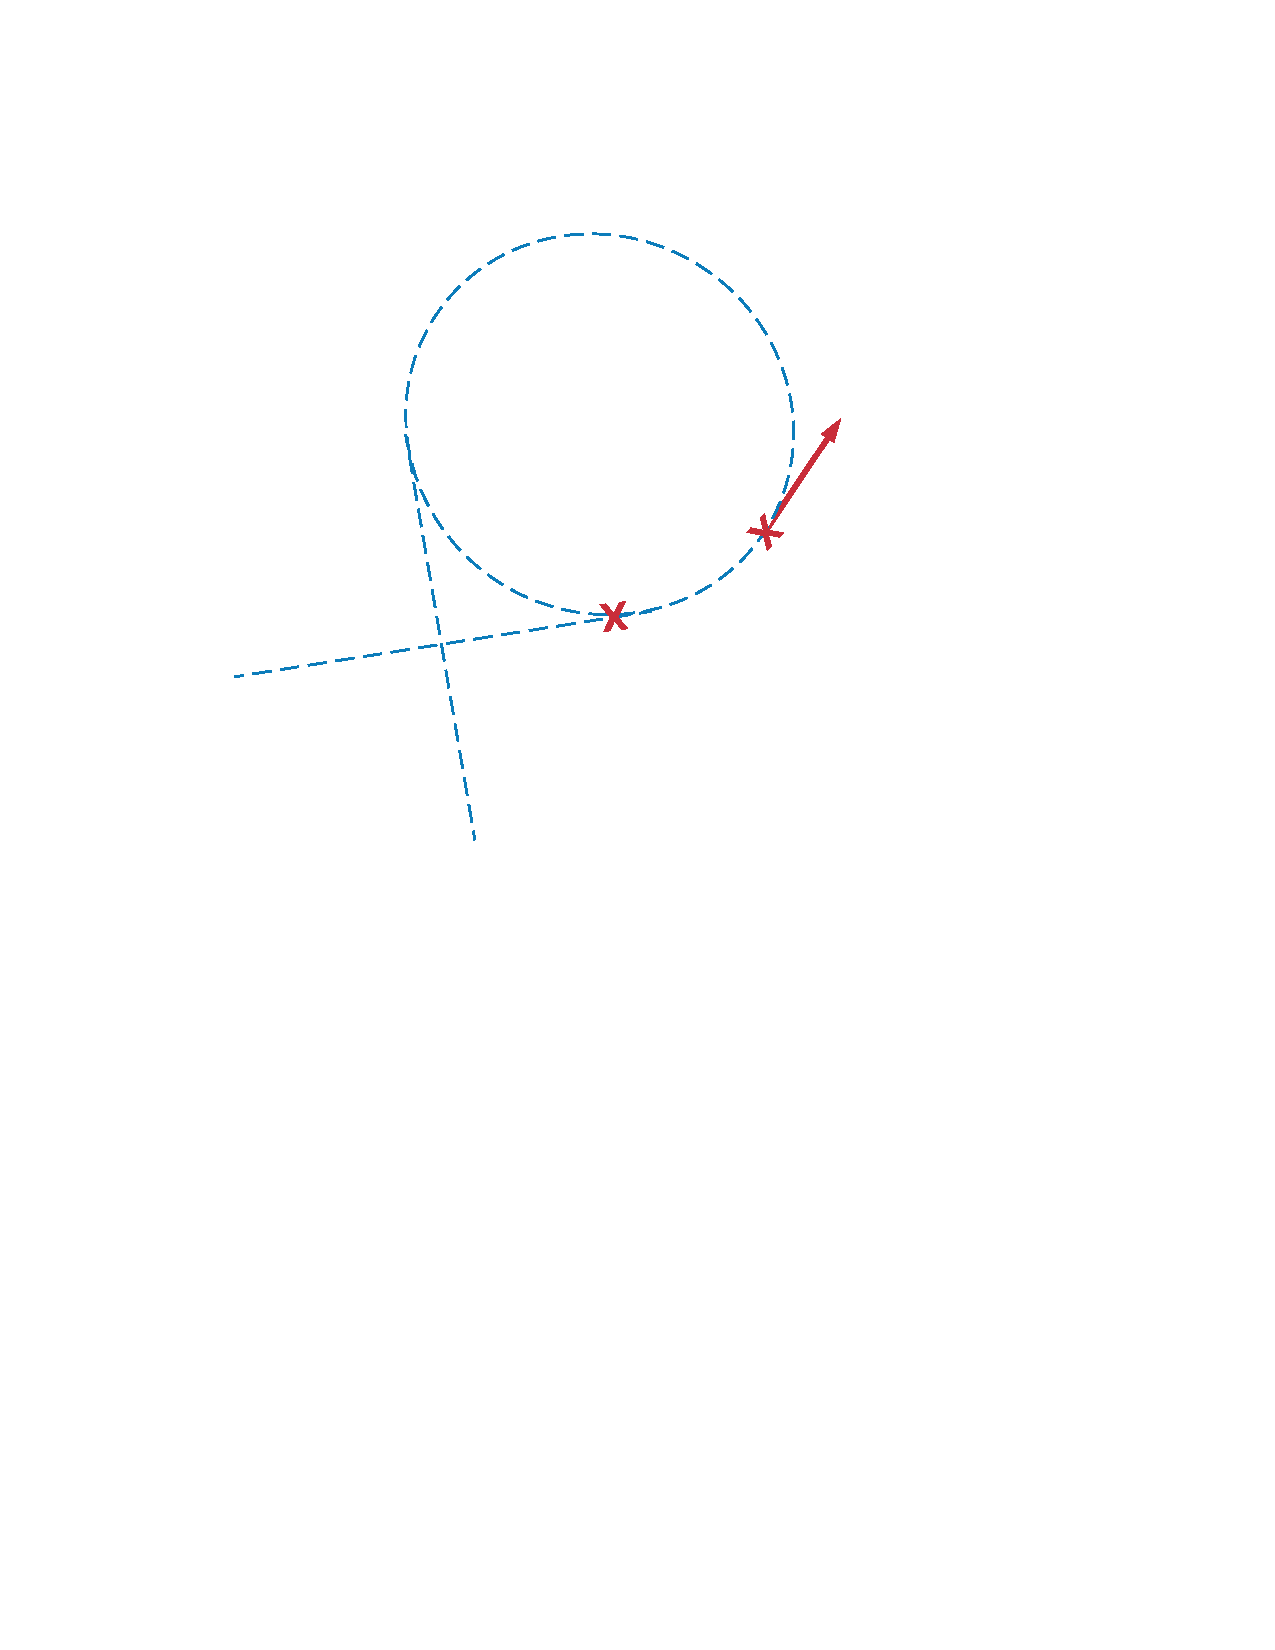
\includegraphics[width=\textwidth]{img/circular_movment1.pdf}
        \caption{Red cross with arrow: state a $t_0$. Red arrow: current velocity vector. Red cross: previous position a $t_{-\alpha}$.}
        \label{fig:one}
   \end{subfigure}\hfill
   \begin{subfigure}[b]{0.45\textwidth}
        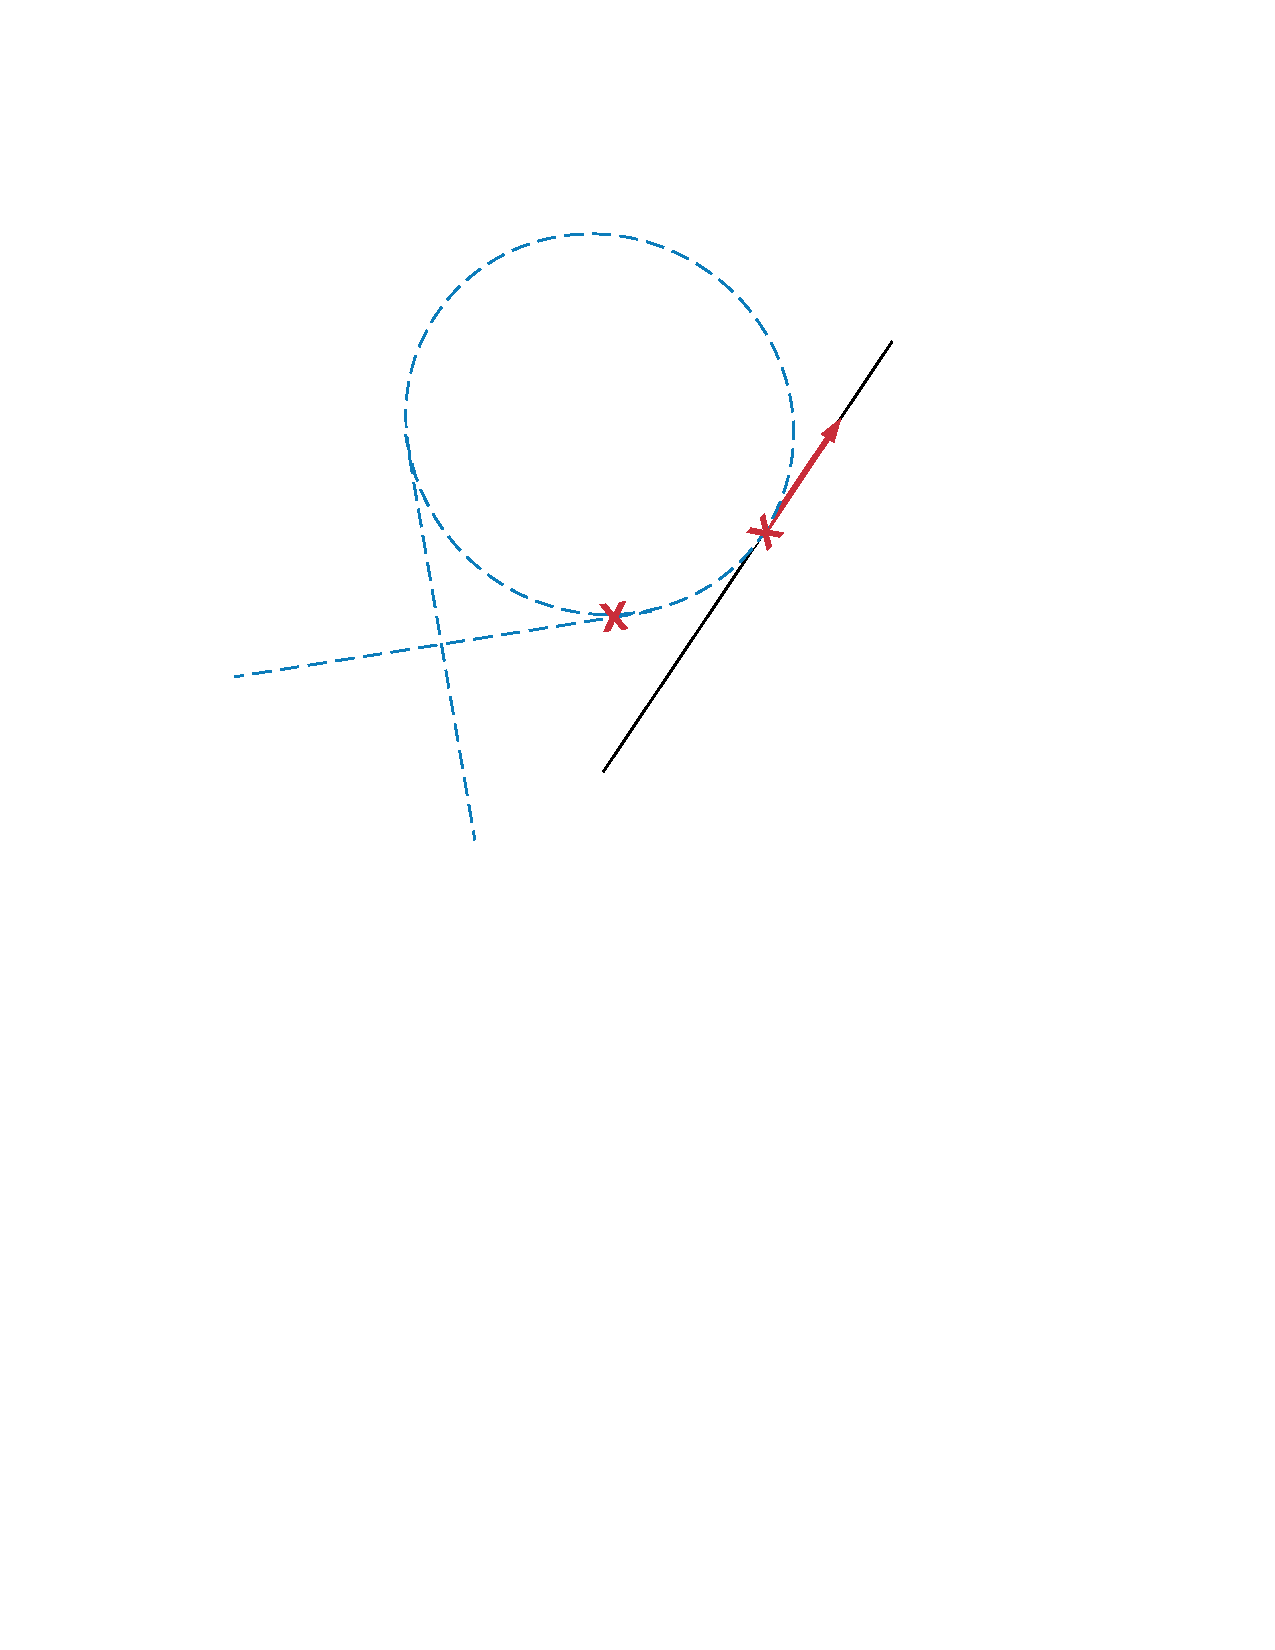
\includegraphics[width=\textwidth]{img/circular_movment2.pdf}
        \caption{Black line: direction of the velocity vector, with angle $\theta_0$. We have symmetry with respect to this axes.}
        \label{fig:two}
   \end{subfigure}
   
   \begin{subfigure}[b]{0.45\textwidth}
        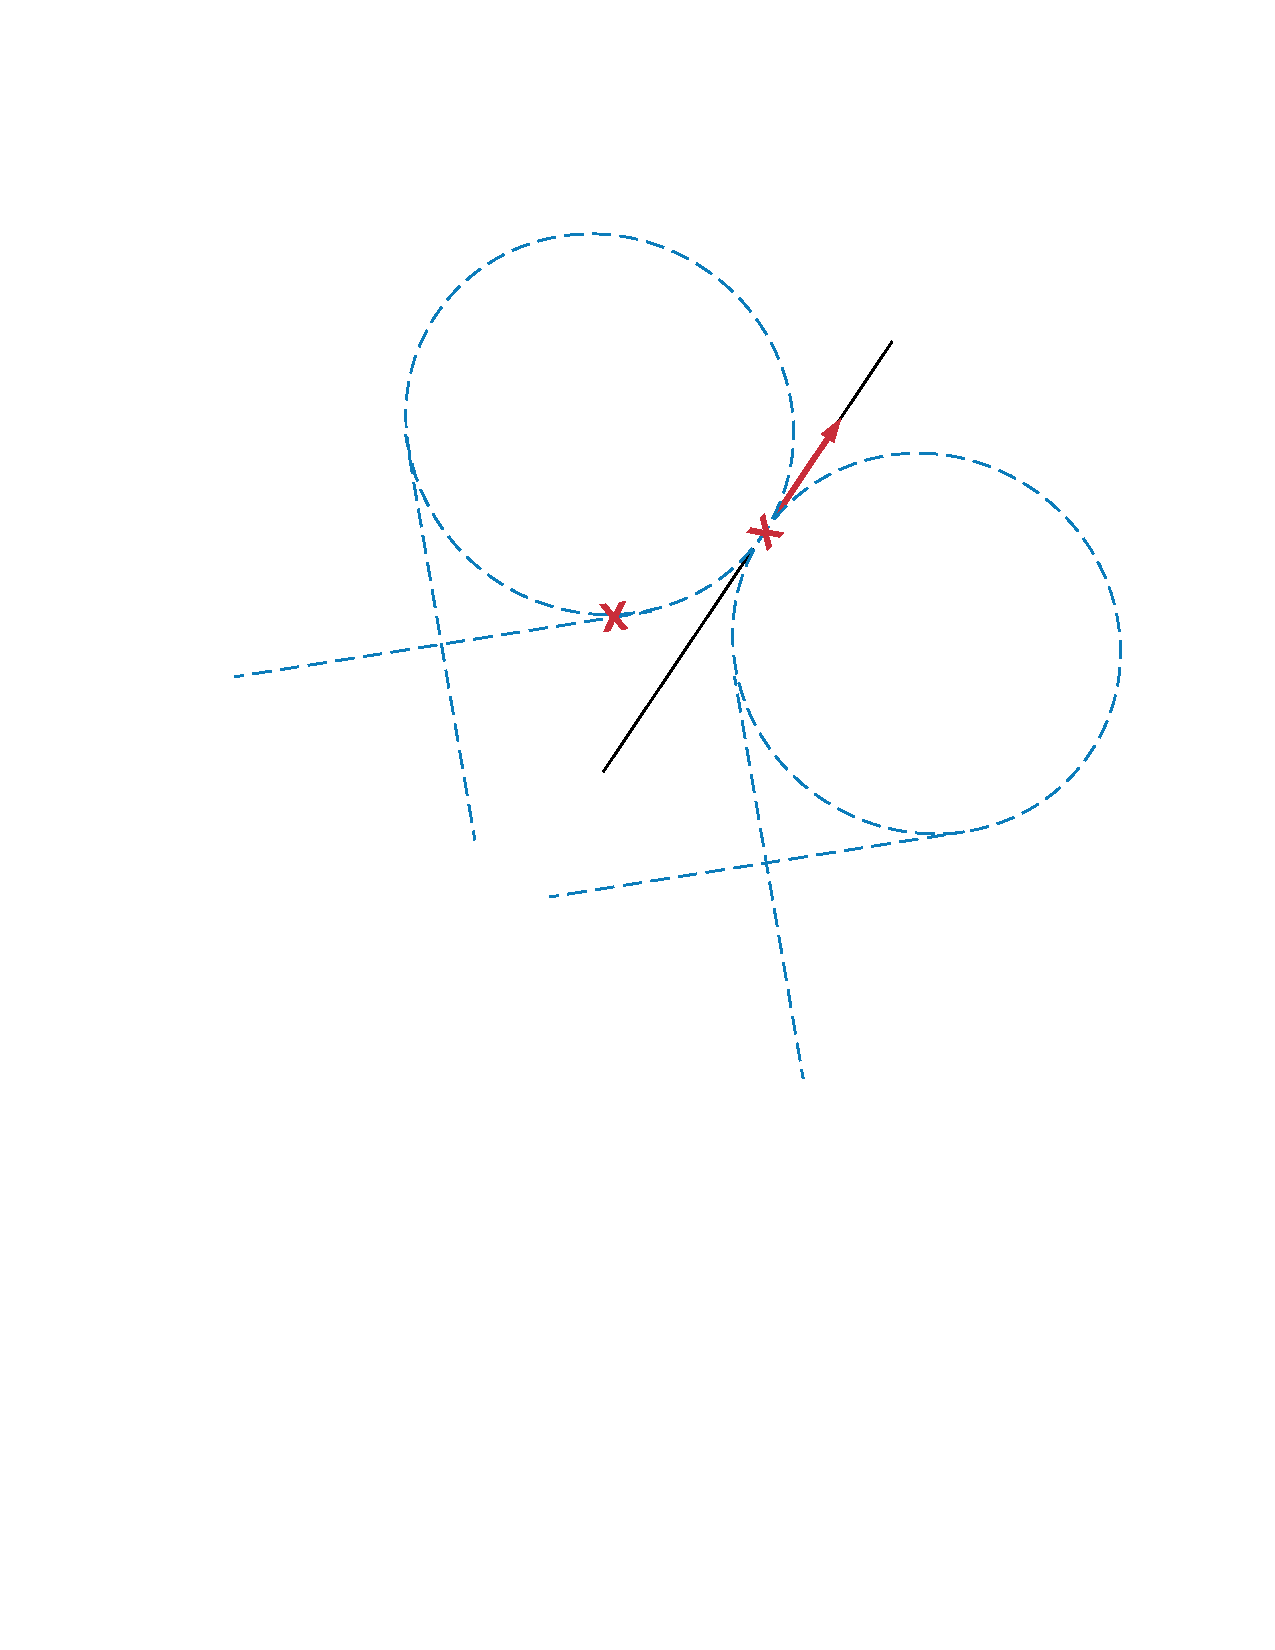
\includegraphics[width=\textwidth]{img/circular_movment3.pdf}
        \caption{Blue lines: real and symmetric path. We do not know which of the two trajectories is correct.}
        \label{fig:three}
   \end{subfigure}\hfill
    \begin{subfigure}[b]{0.45\textwidth}
        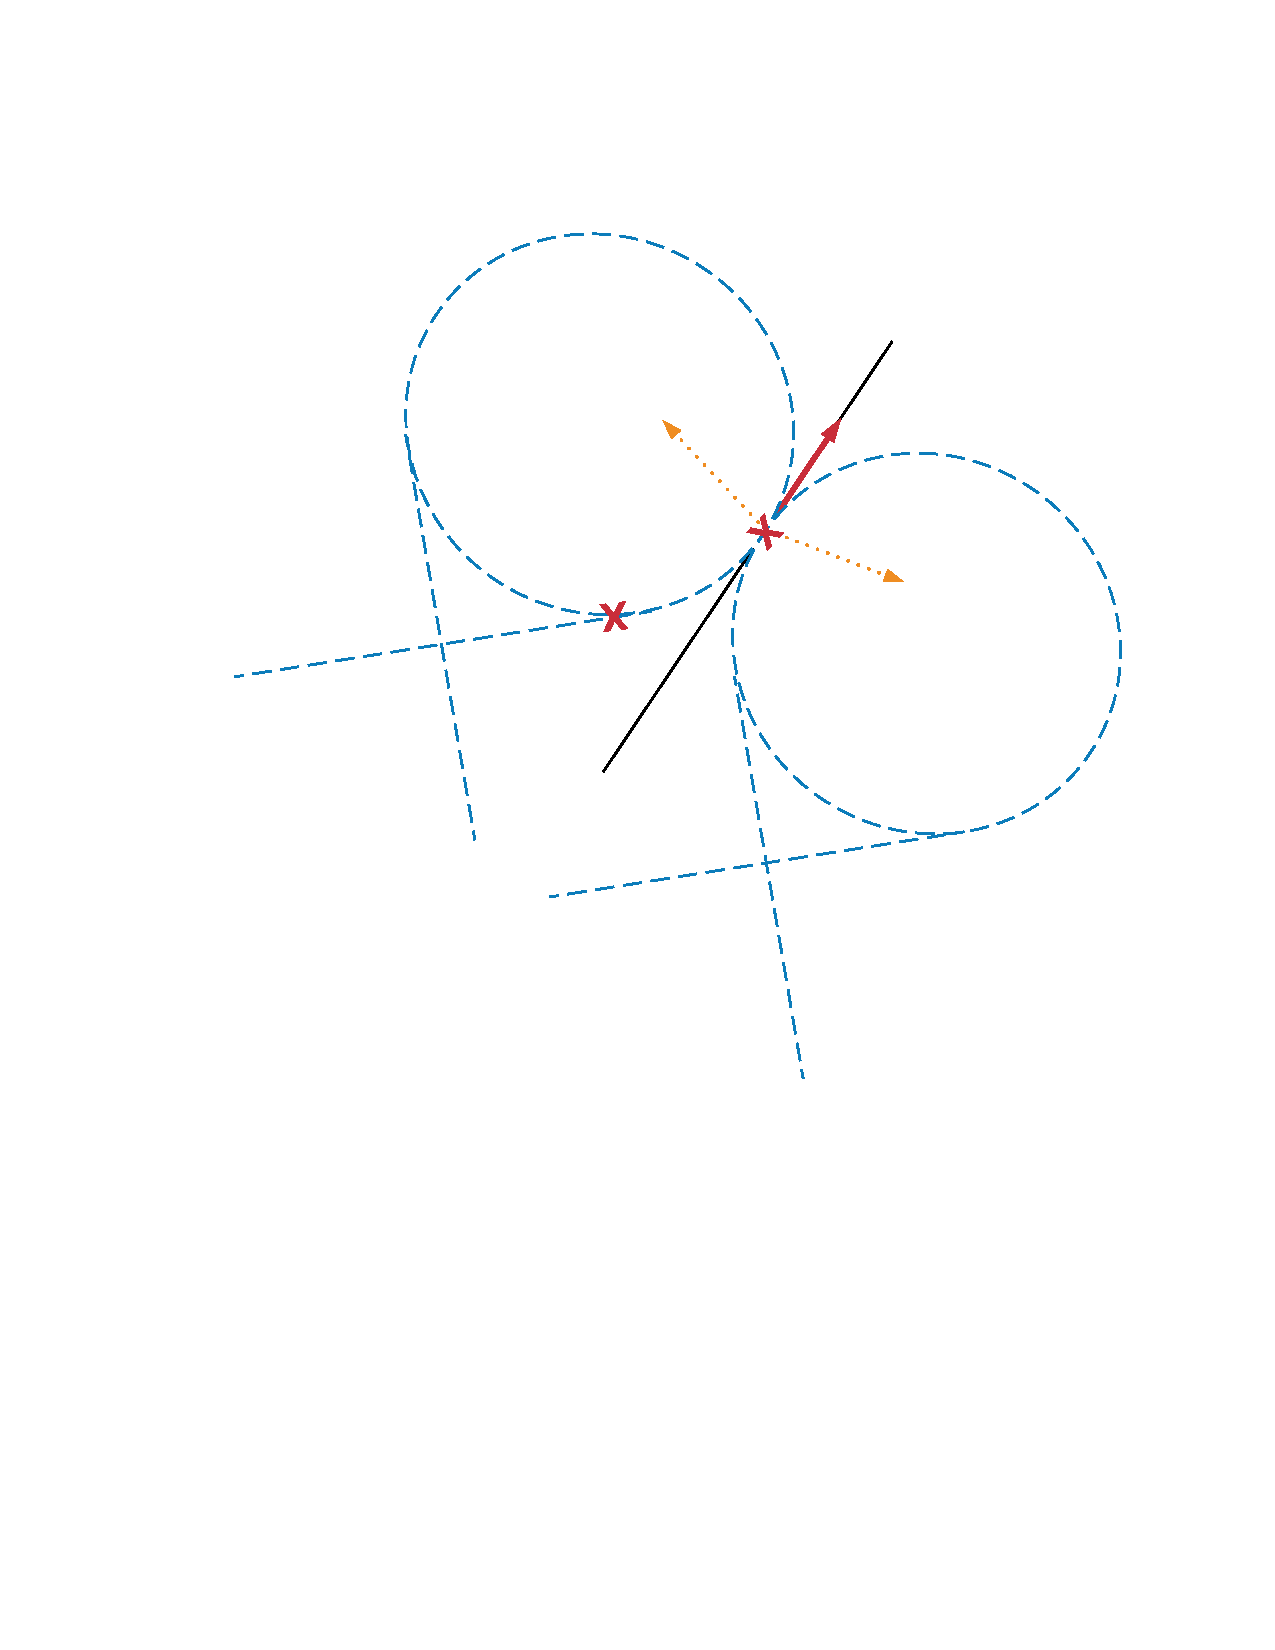
\includegraphics[width=\textwidth]{img/circular_movment4.pdf}
        \caption{Yellow arrows: estimated future angles $\theta_1^a$ and $\theta_1^b$ that the base will assume at time $t_1$.}
        \label{fig:four}
   \end{subfigure}
   
    \begin{subfigure}[b]{0.45\textwidth}
        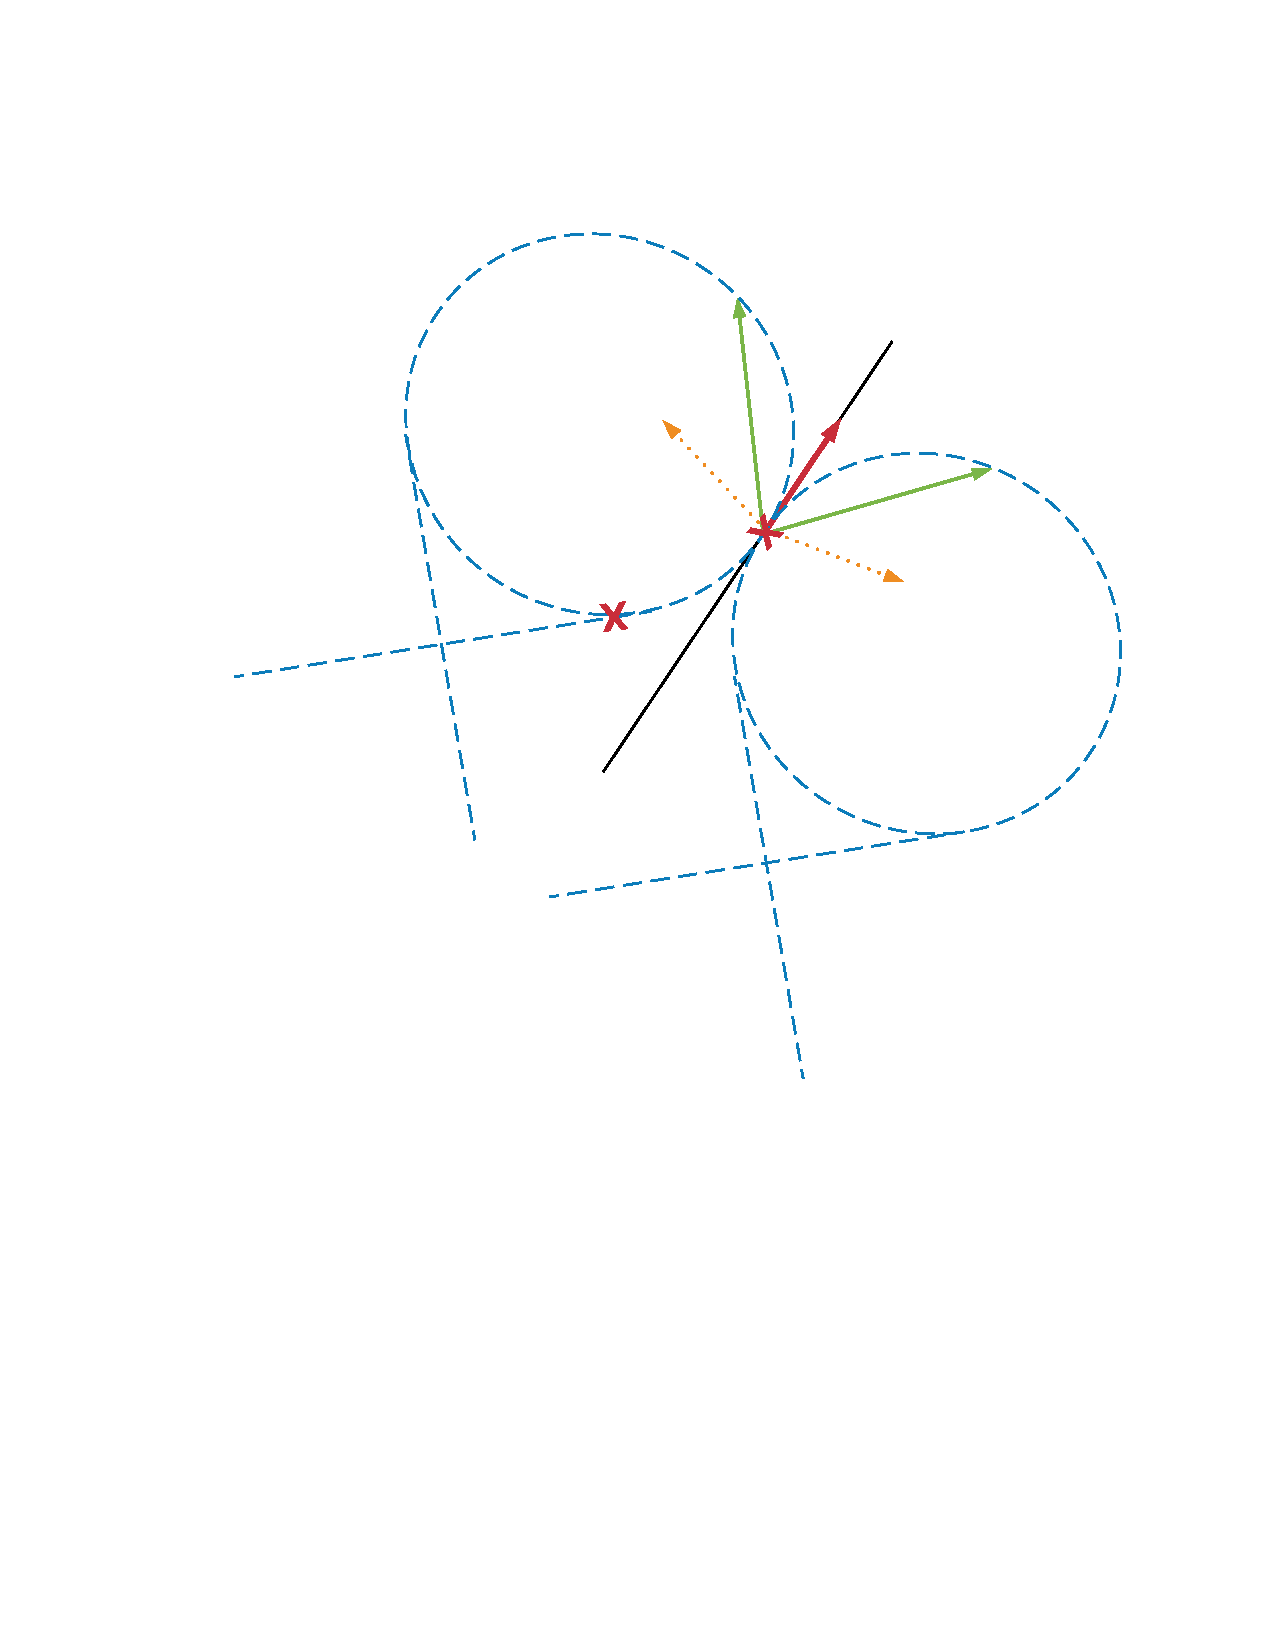
\includegraphics[width=\textwidth]{img/circular_movment5.pdf}
        \caption{Green arrows: segment from state at $t_0$ and possible states at $t_1$: with angles $\theta_{chord}^a$  and $\theta_{chord}^b$ and length $l_{chord}$ }
        \label{fig:five}
   \end{subfigure}\hfill
    \begin{subfigure}[b]{0.45\textwidth}
        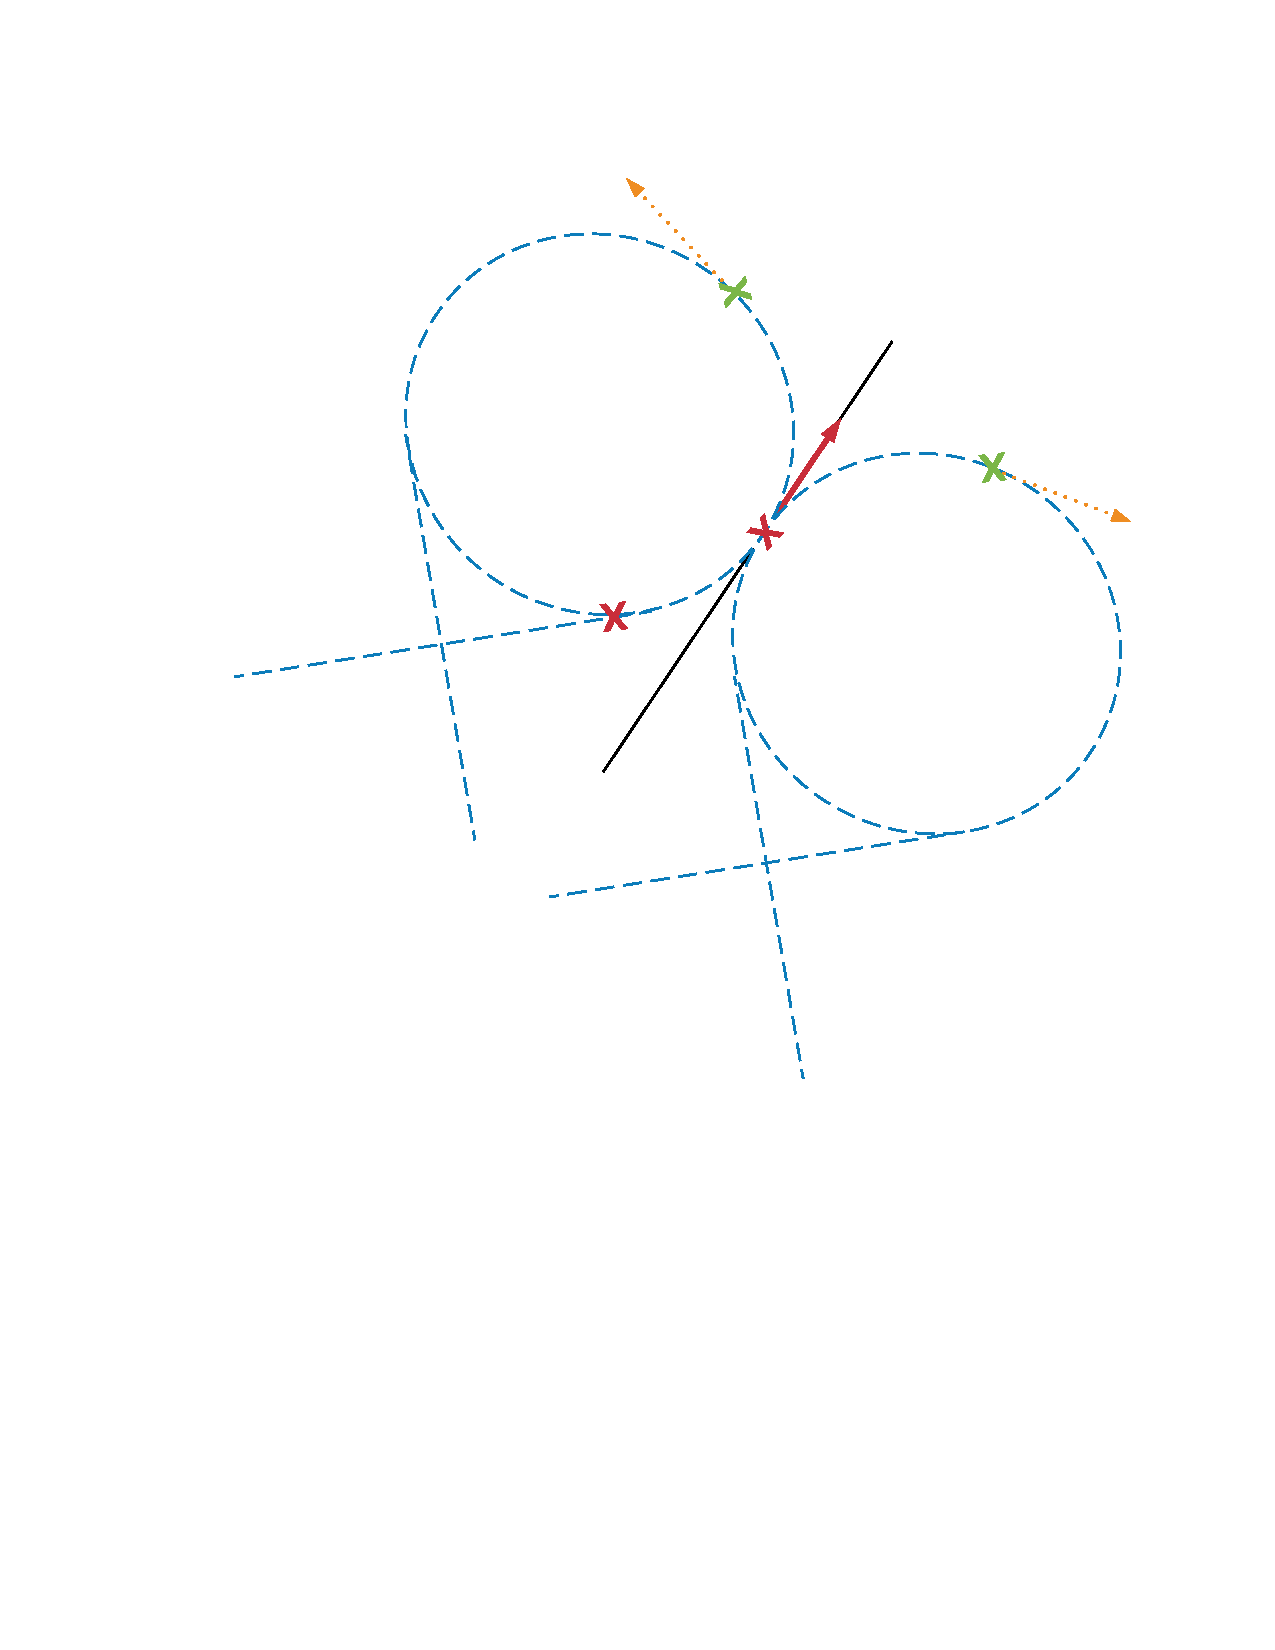
\includegraphics[width=\textwidth]{img/circular_movment6.pdf}
        \caption{Green crosses: future possible states of the platform at positions $(x_1^a,y_1^a)$ and $(x_1^b,y_1^b)$ .}
        \label{fig:six}
   \end{subfigure}
   
    \begin{subfigure}[b]{0.45\textwidth}
        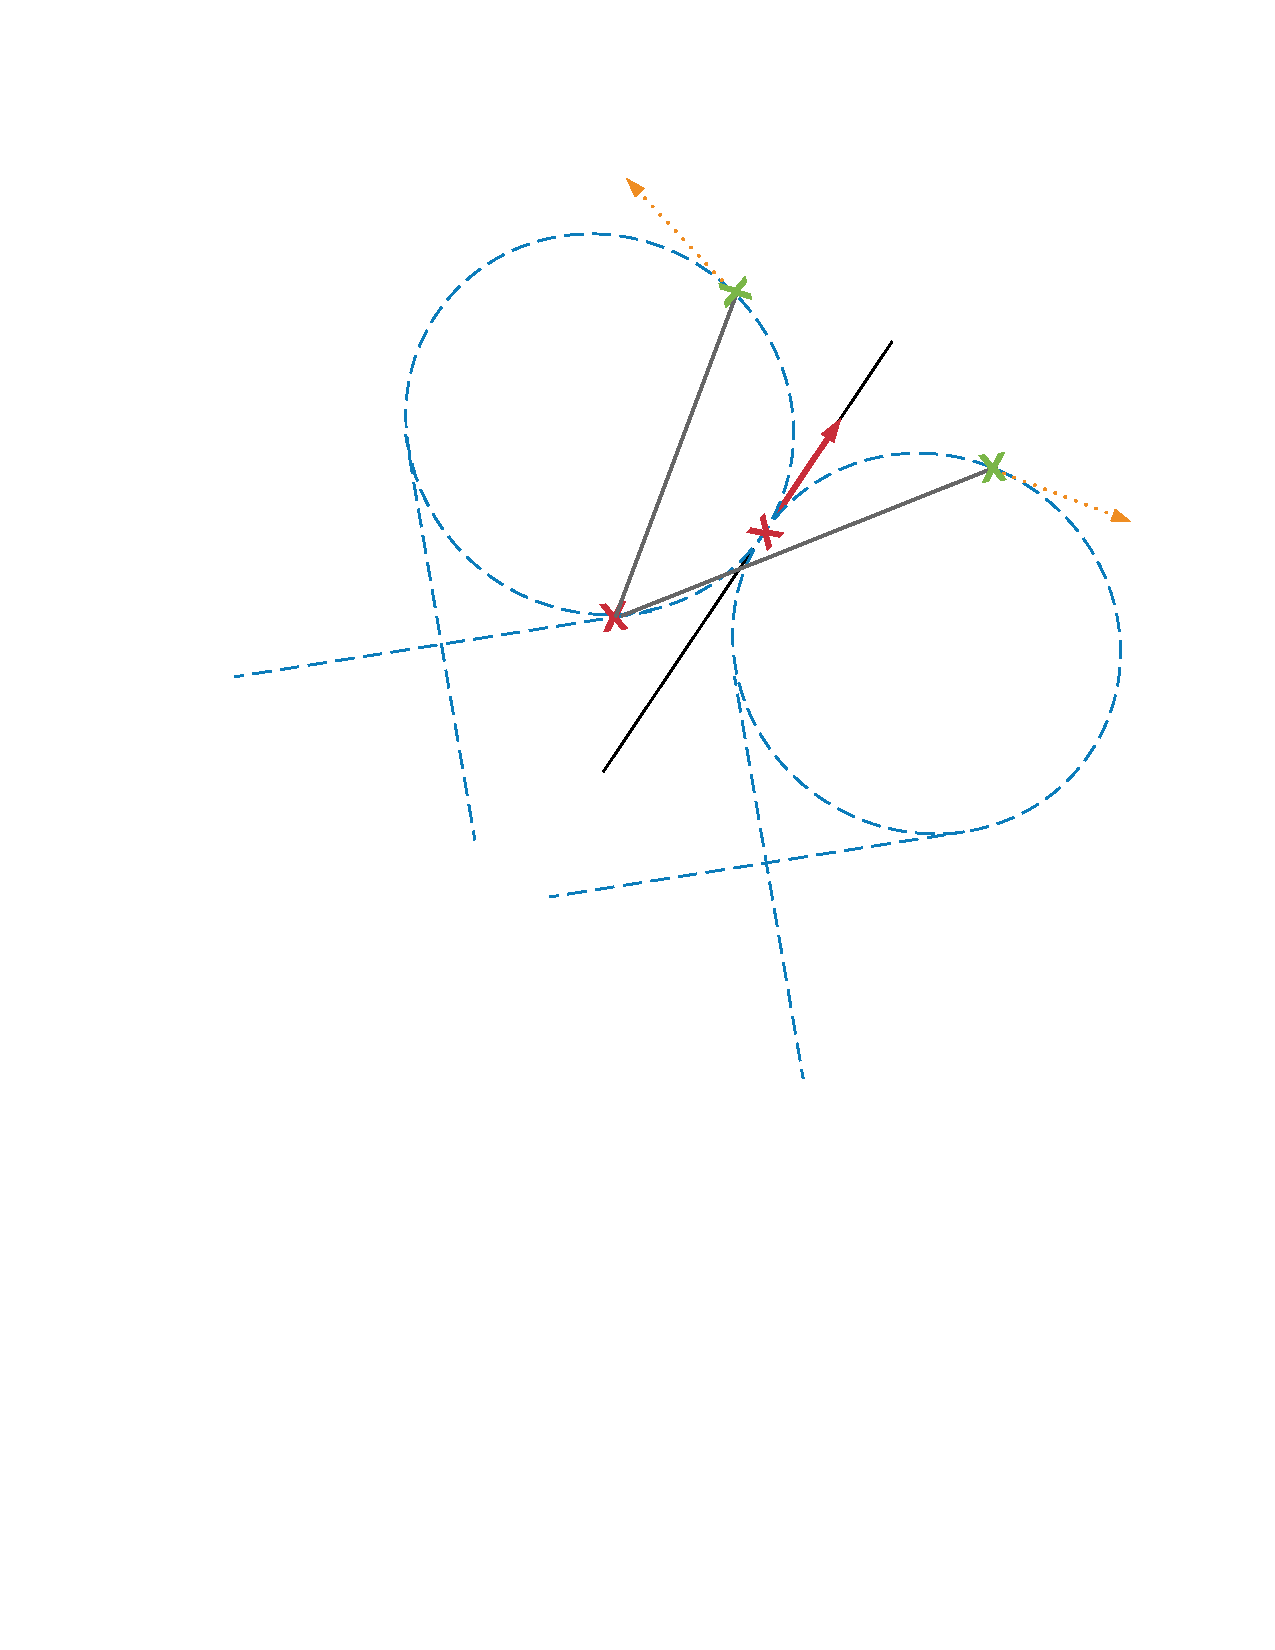
\includegraphics[width=\textwidth]{img/circular_movment7.pdf}
        \caption{Dark grey lines: distances from previous position at $t_{-\alpha}$ and possible future positions at $t_1$. }
        \label{fig:seven}
   \end{subfigure}\hfill
    \begin{subfigure}[b]{0.45\textwidth}
        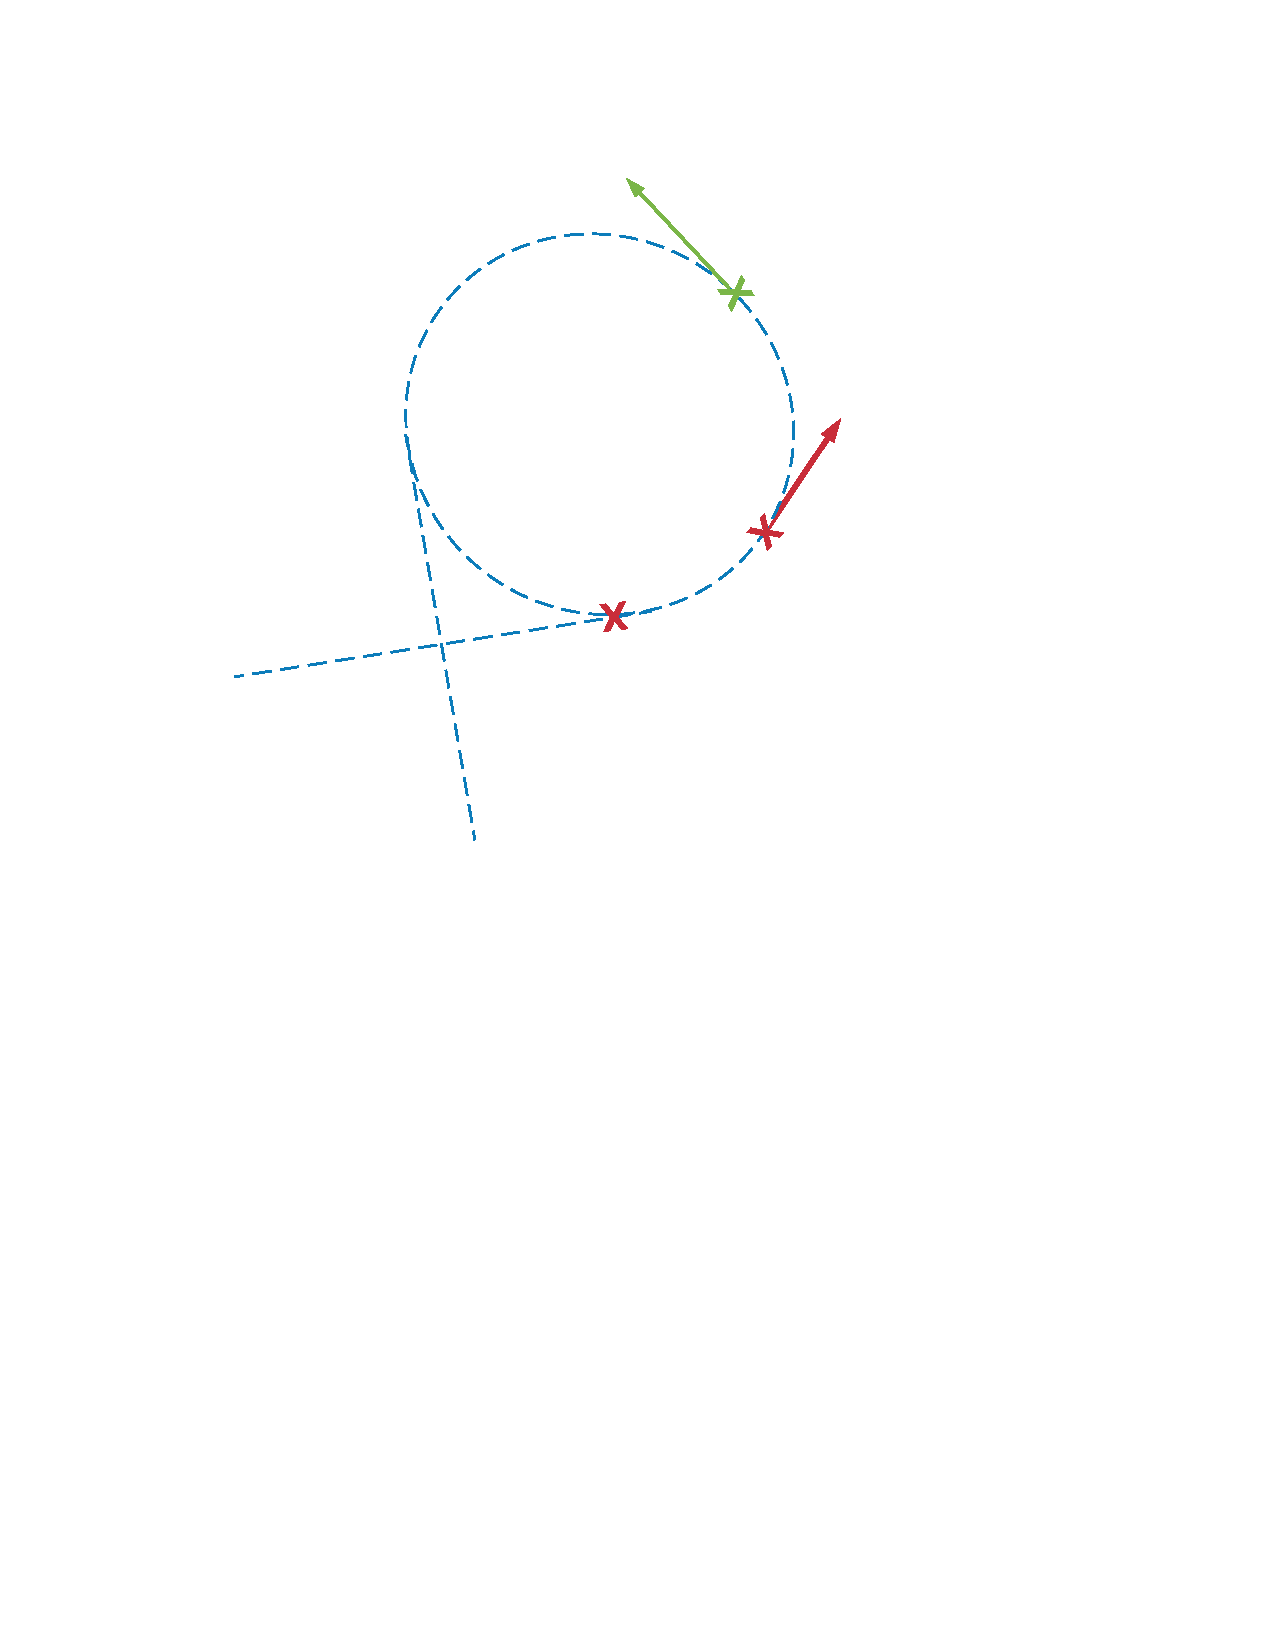
\includegraphics[width=\textwidth]{img/circular_movment8.pdf}
        \caption{Green cross with arrow: future state selected taking the position with minimum distance.}
        \label{fig:eight}
   \end{subfigure}
  \caption{The sequence of passages computed in order to select the future position when the platform is moving on the circumference.}
  \label{fig:sequence_find_next_position_circumference}
\end{figure} 
\end{itemize}
The image \ref{fig:map_waypoints} shows where the algorithm calculates the way points for the quadrotor in order to following the moving car.

\begin{figure}[!htbp]
    \centering
    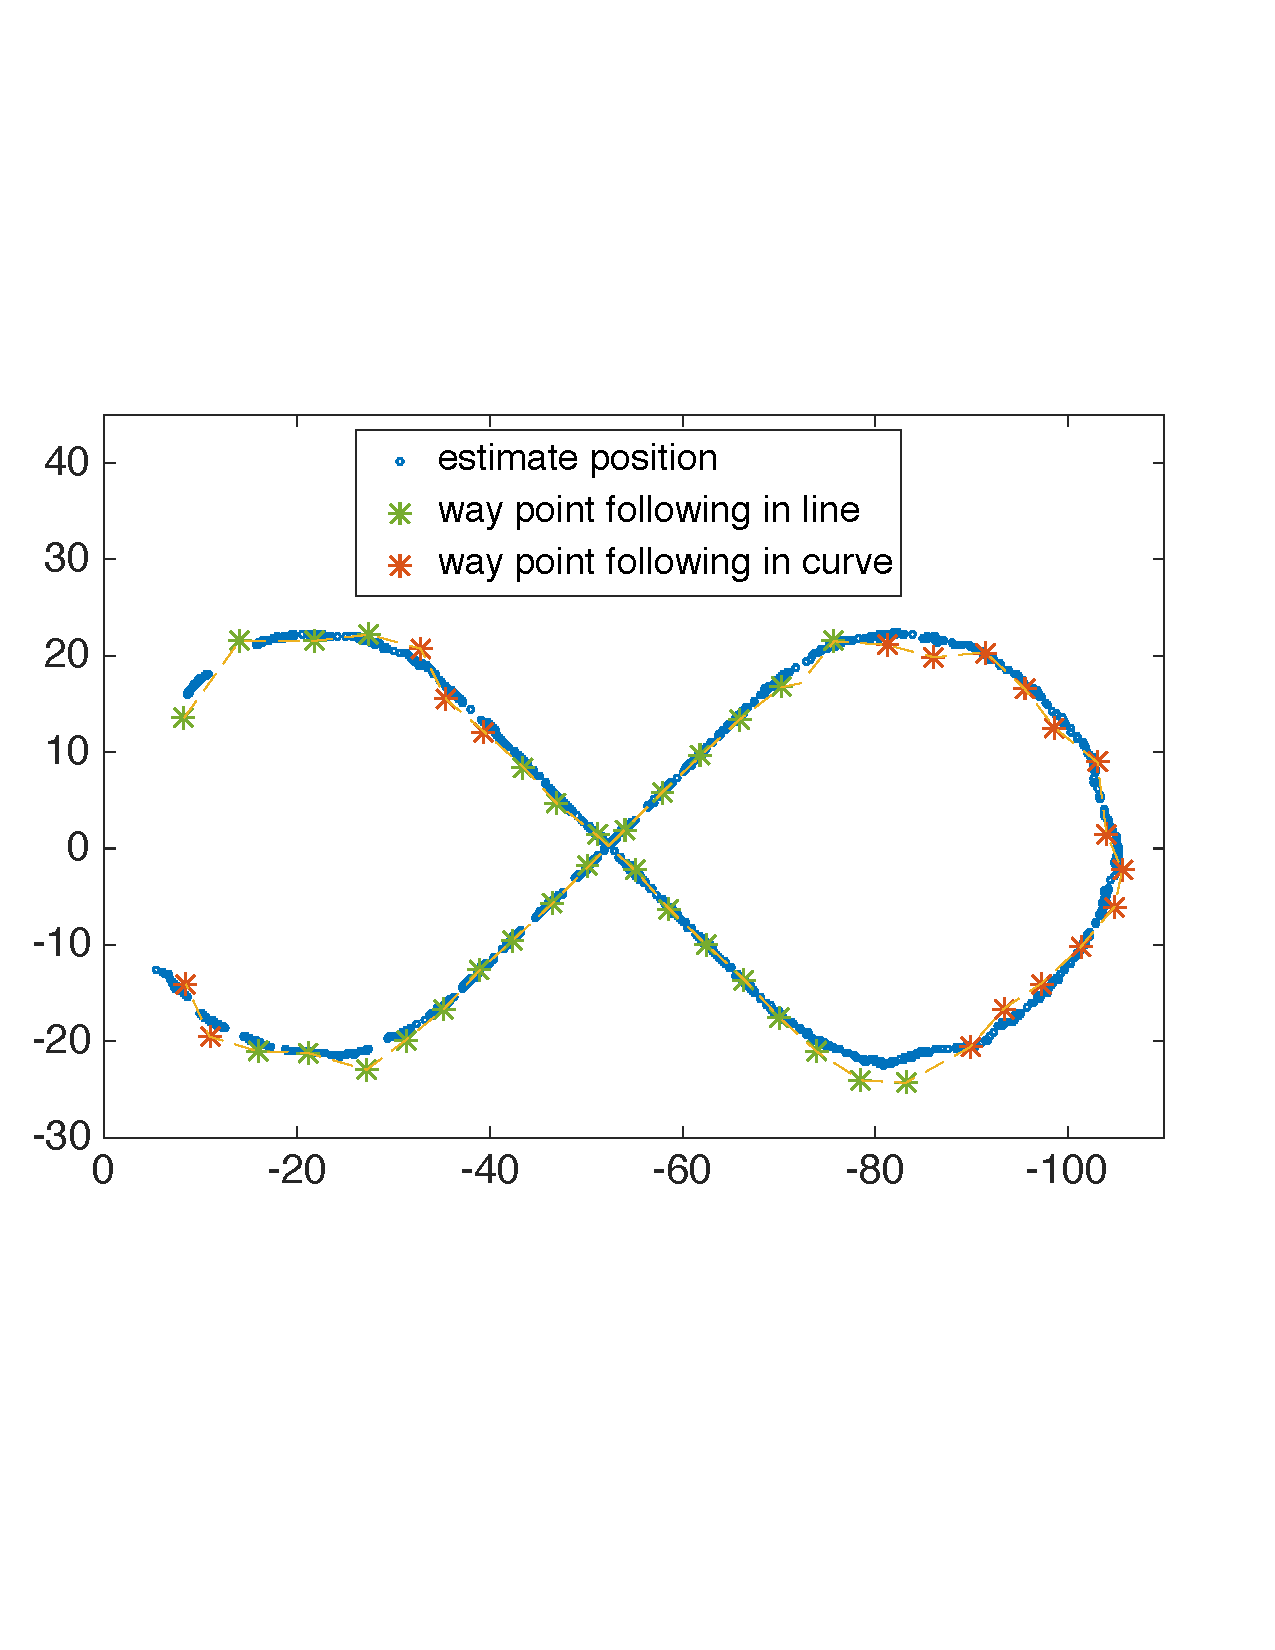
\includegraphics[width=1.0\textwidth]{img/following_platform_long_map_waypoints.pdf}
    \caption{Data from the first phase of the area exploration. Blue circles position of the base estimate. Stars the position in which the quadrotor should go to following the base until a proper moment to proceed with the following phases is detected. }
    \label{fig:map_waypoints}
\end{figure}

\subsubsection{Following the base and proceed with following phase}
At this point we can use the predict position of the platform to control the quadrotor in order to following the base and at the right moment proceed with the other phases.\\
The right moment to perform the landing is at the start of a line segment:
\begin{itemize}
\item if we first detect the base and we understand that it is moving in a circumference we cannot land, we can follow the base and waiting when we will detect a change in the regime from curve to line. At this point we can proceed with the landing.
\item if we first detect the base and we understand that it is moving in a straight line we should not land, because we do not know when it actually started the line, so it can be almost at the end of it, and we do not have time to perform the entire landing maneuver. What we do is following the car and waiting when it changes from the line movement to the curve. At this point we can calculate where the next change point will be:
\begin{itemize}
\item we know the orientation of the straight line portion just finished and it is $\theta_{line}$
\item given the point of change between line and curve, the future point will be in the circumference after an angle of $\big | \frac{3\pi}{2} \big |$.
\item from equations \ref{eq:anglechord} \ref{eq:lengthchord} we know that the segment connecting the change point and the future intersection point has length $\sqrt{2}r_8$ and angle $\theta_{line} \pm \frac{3\pi}{4} $
\item we can apply the same method described before to find the two possible intersection points:
\begin{align}
\begin{cases}
x_{intersection}^a &= x_{changing} + \sqrt{2}r_8\cos{\Big(\theta_{line} + \frac{3\pi}{4}\Big) }\\
y_{intersection}^a &= y_{changing} + \sqrt{2}r_8\sin{\Big(\theta_{line} + \frac{3\pi}{4}\Big) }\\
\theta_{intersection}^a &=  \theta_{line} + \frac{3\pi}{2}
\label{eq:finalstatecurveb}
\end{cases}
\end{align}

\begin{align}
\begin{cases}
x_{intersection}^b &= x_{changing} + \sqrt{2}r_8\cos{\Big(\theta_{line} - \frac{3\pi}{4}\Big) }\\
y_{intersection}^b &= y_{changing} + \sqrt{2}r_8\sin{\Big(\theta_{line} - \frac{3\pi}{4}\Big) }\\
\theta_{intersection}^b &=  \theta_{line} - \frac{3\pi}{2}
\label{eq:finalstatecurveb}
\end{cases}
\end{align}
and select the right one with minimum distance with the current estimate position of the platform.
The images  \ref{fig:sequence_find_next_intersection} show all the passages we perform to find the right intersection point.
\end{itemize}
Now that we know where the next change of regime will be, we can follow the base and continue with the following phases when the base is close to the intersection point.

\begin{figure}[!htbp]
  \centering
   \begin{subfigure}[b]{0.45\textwidth}
        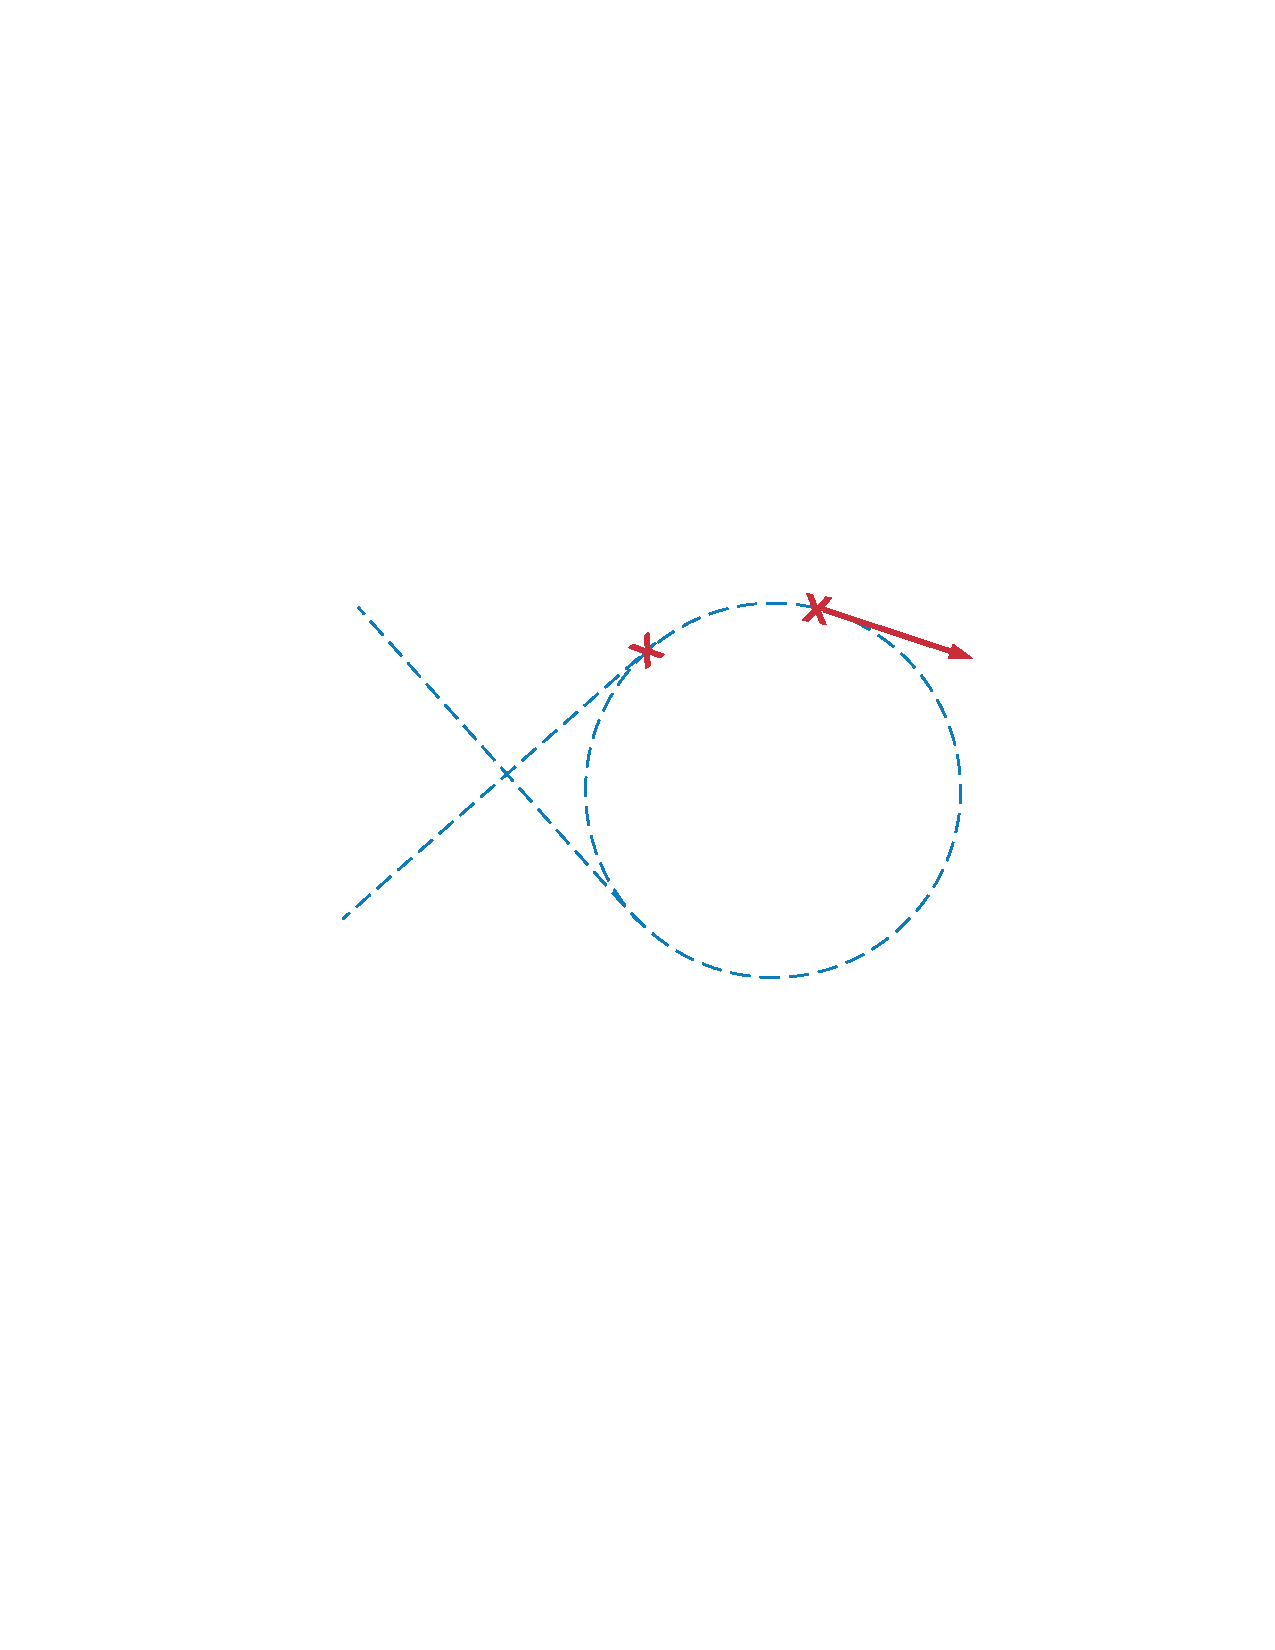
\includegraphics[width=\textwidth]{img/intersection_1.pdf}
        \caption{Red cross with arrow: state a $t_0$. Red arrow: current velocity vector. Red cross: changing point from line to curve.}
        \label{fig:one}
   \end{subfigure}\hfill
   \begin{subfigure}[b]{0.45\textwidth}
        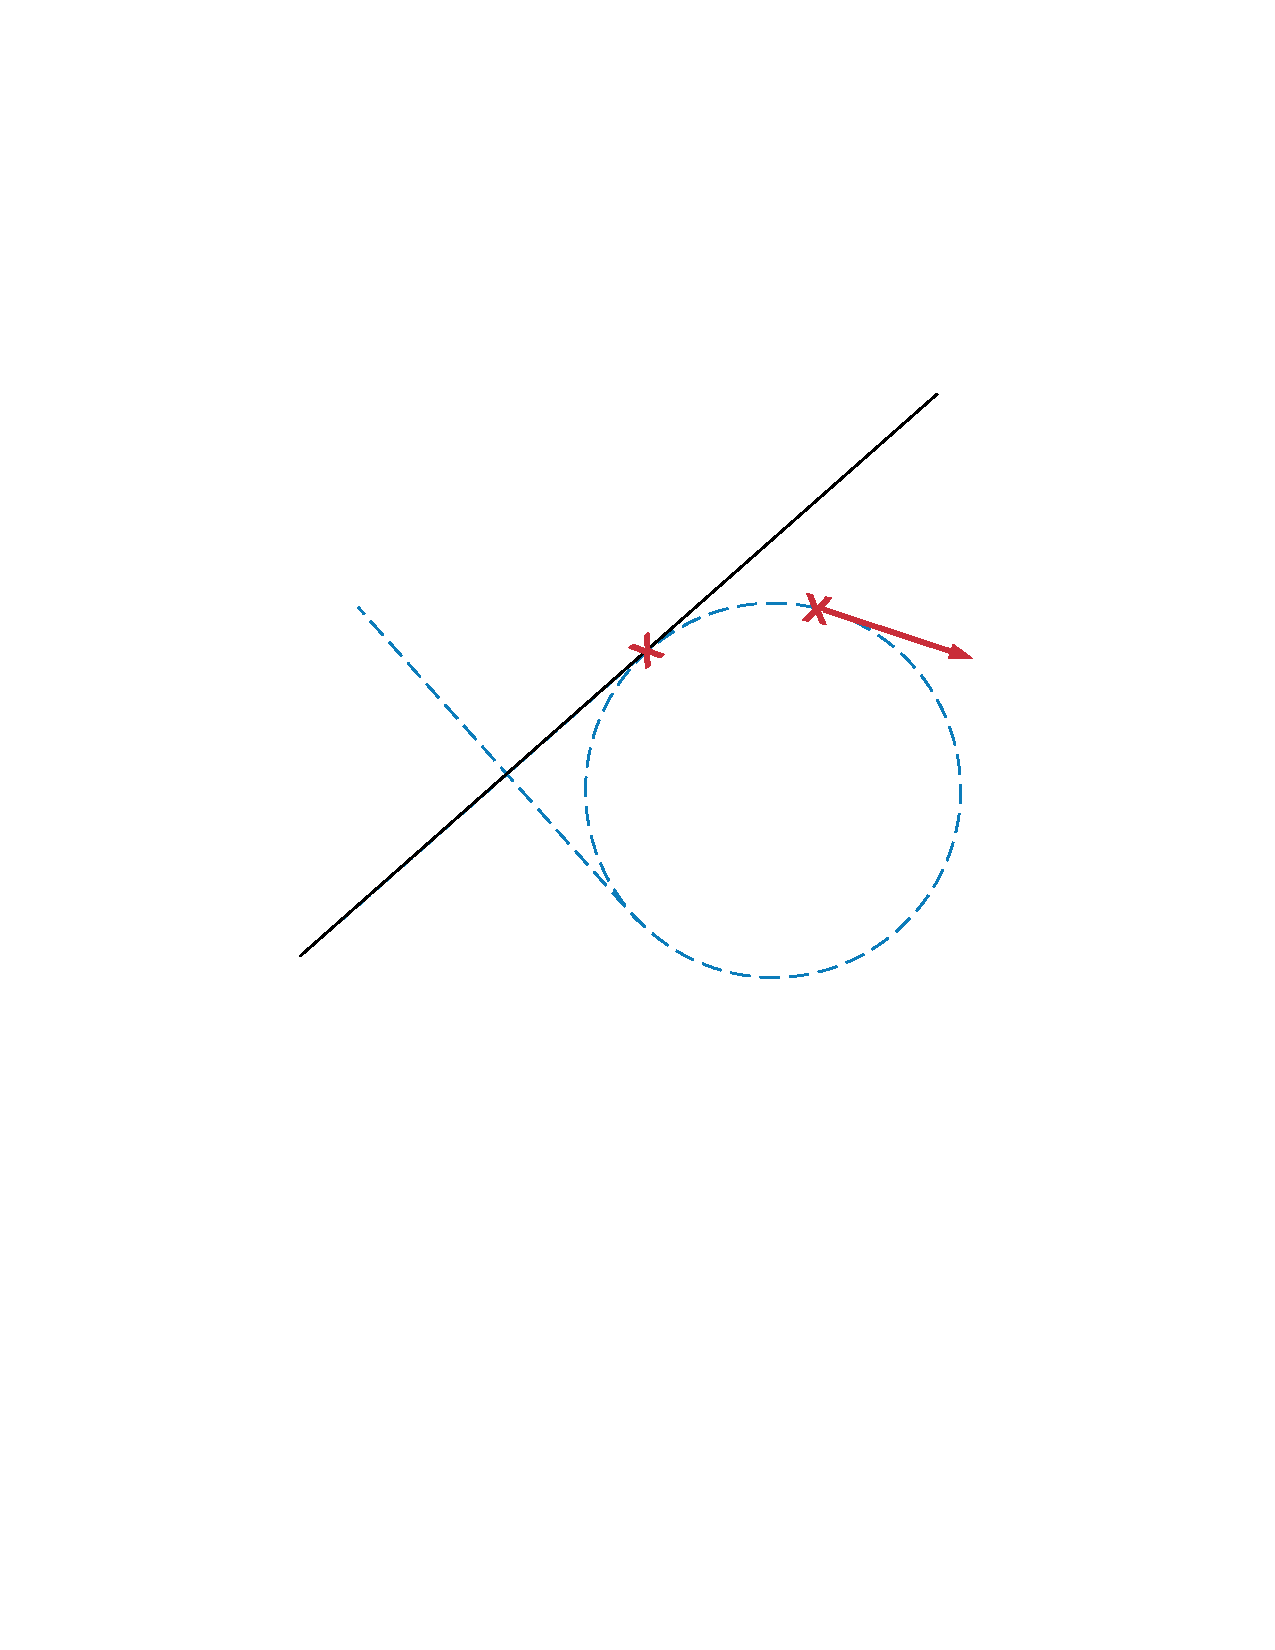
\includegraphics[width=\textwidth]{img/intersection_2.pdf}
        \caption{Black line: direction of the line sector just finished. The direction is taken as the slope of the best linear fit found in the previous regime.}
        \label{fig:two}
   \end{subfigure}
   
   \begin{subfigure}[b]{0.45\textwidth}
        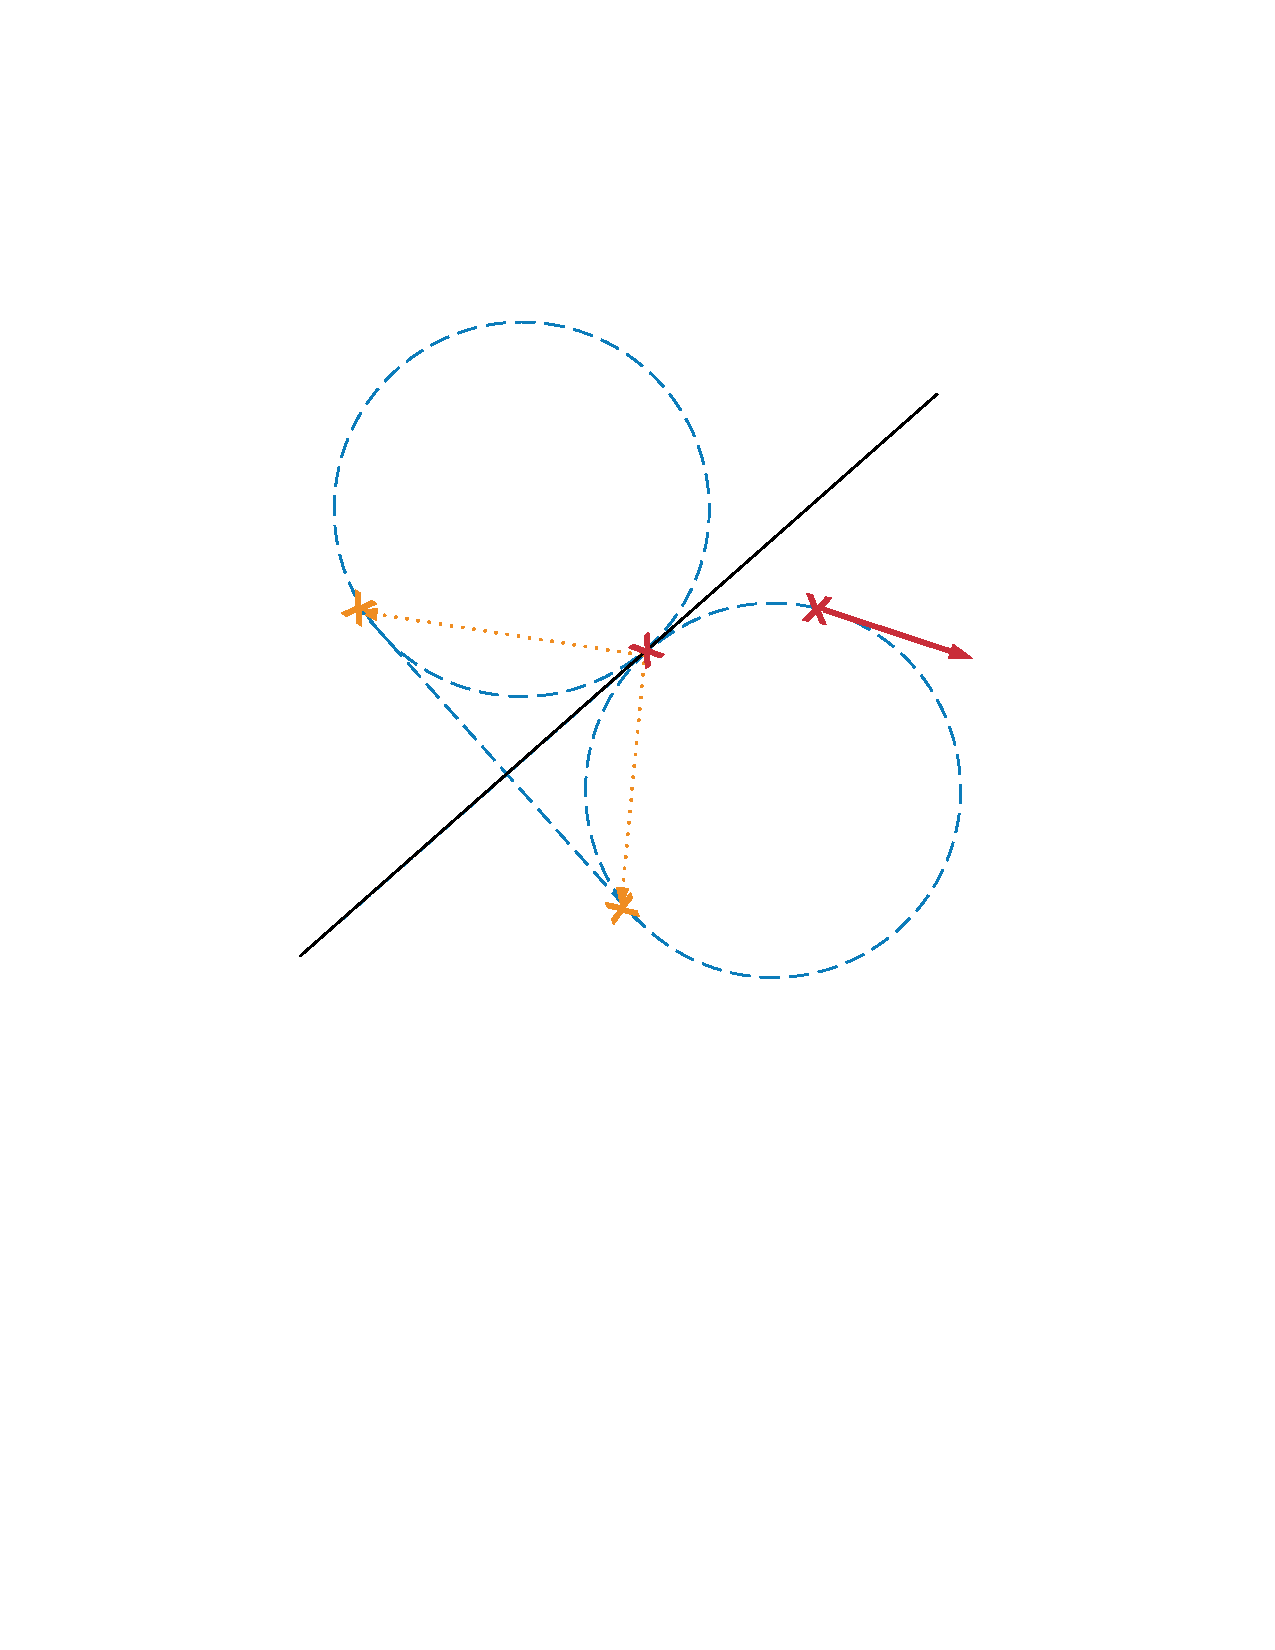
\includegraphics[width=\textwidth]{img/intersection_3.pdf}
        \caption{Blue lines: real and symmetric path. We do not know which of the two trajectories is correct. Yellow crosses: in both the path we can calculate the future intersection point.}
        \label{fig:three}
   \end{subfigure}\hfill
    \begin{subfigure}[b]{0.45\textwidth}
        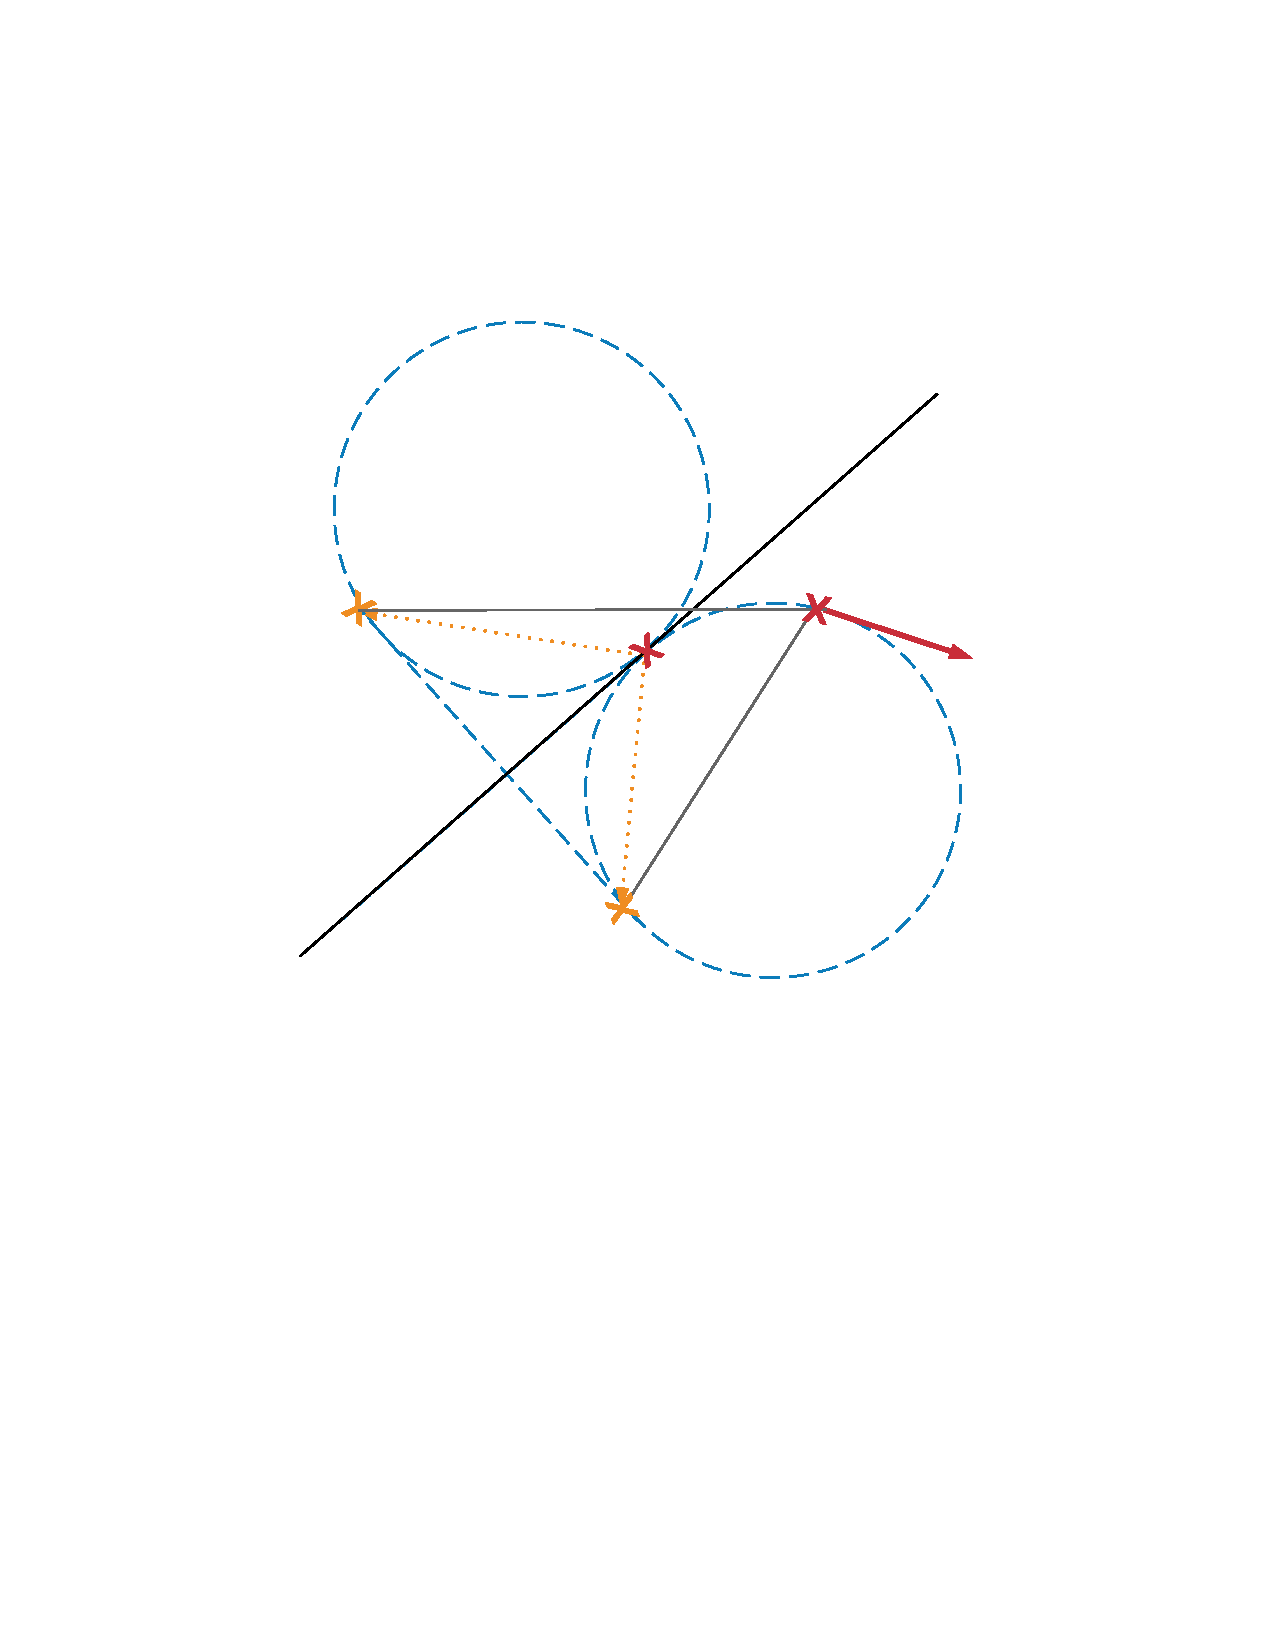
\includegraphics[width=\textwidth]{img/intersection_4.pdf}
        \caption{Dark grey lines: distances from current position and the two possible future intersections. Both are eligible becouse of the symmetry of the trajectory.}
        \label{fig:four}
   \end{subfigure}
   
    \begin{subfigure}[b]{0.45\textwidth}
        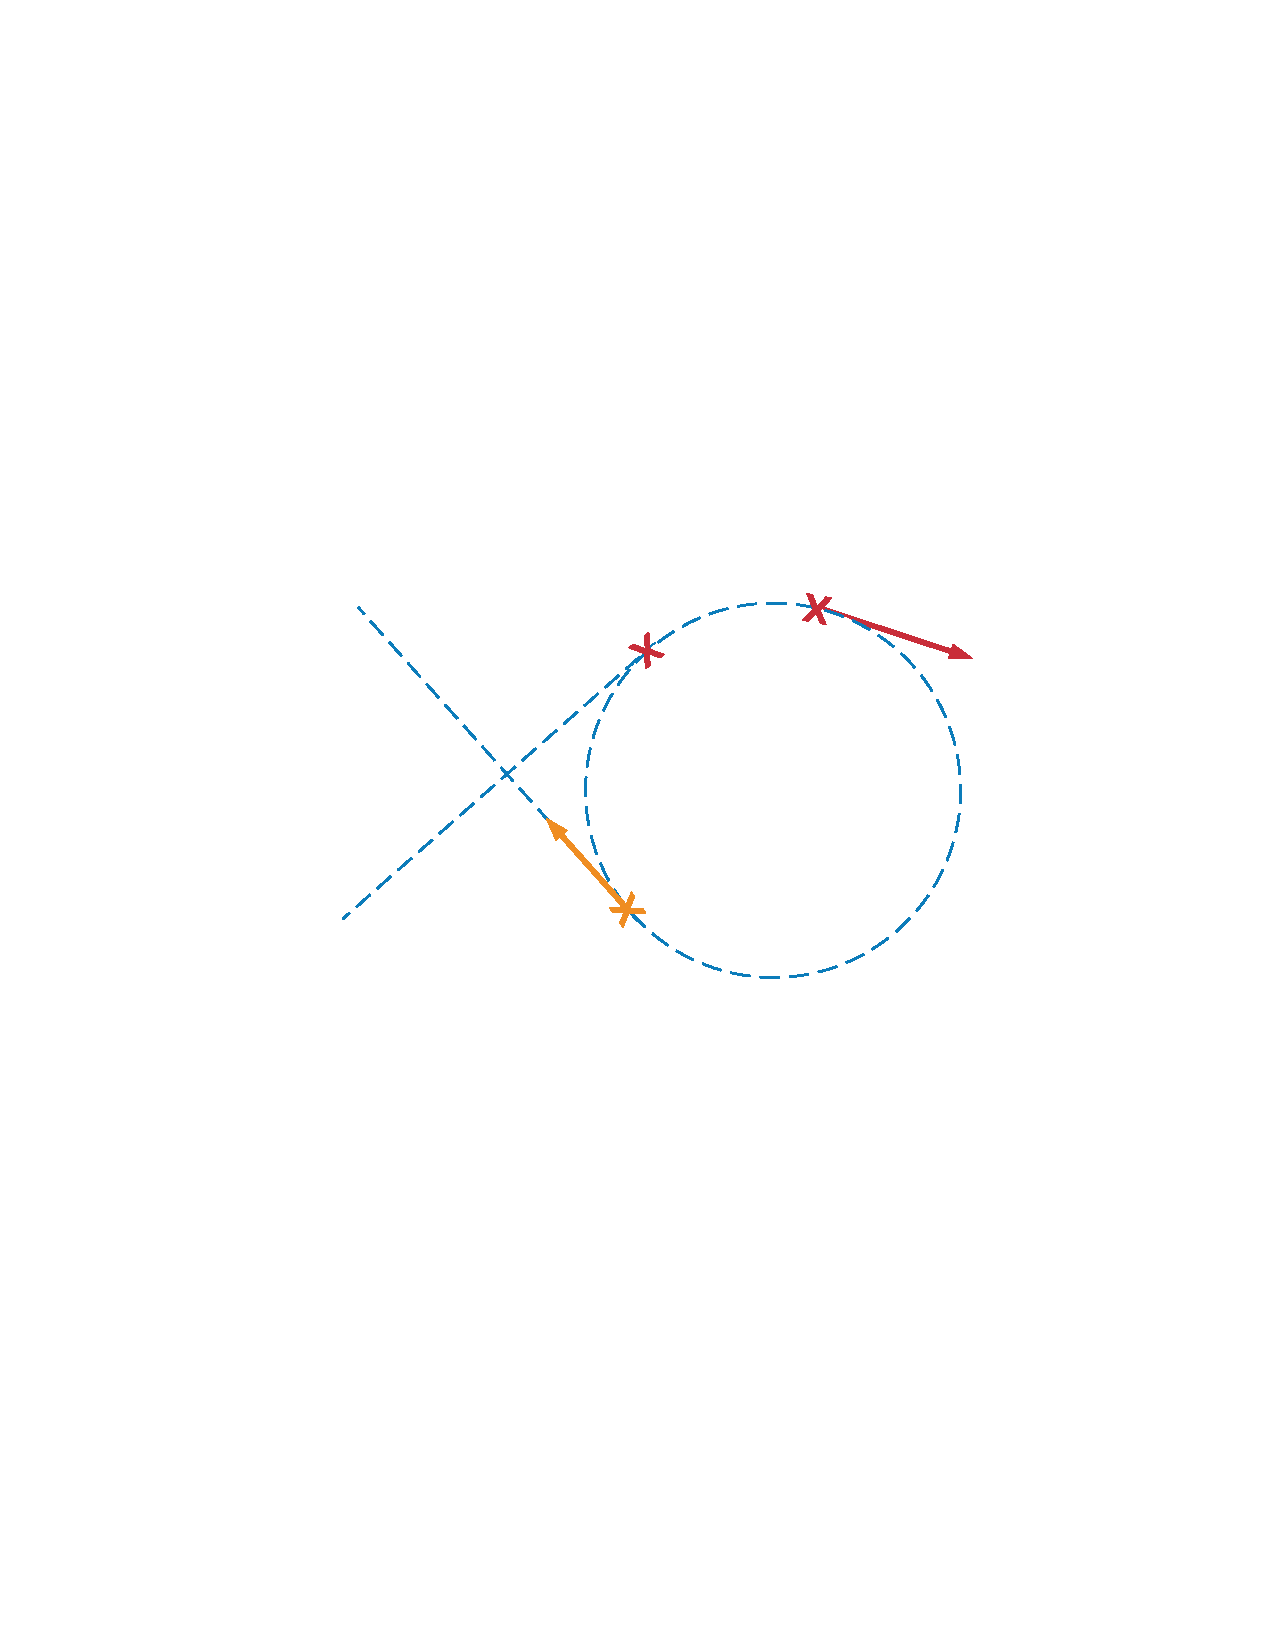
\includegraphics[width=\textwidth]{img/intersection_5.pdf}
        \caption{Yellow cross with arrow: future intersection point selected taking the position with minimum distance from the current state. }
        \label{fig:five}
   \end{subfigure}
  \caption{The sequence of passages computed in order to select the future intersection point where the platform will start the movement in line.}
  \label{fig:sequence_find_next_intersection}
\end{figure} 

\end{itemize}


\begin{figure}[!htbp]
    \centering
    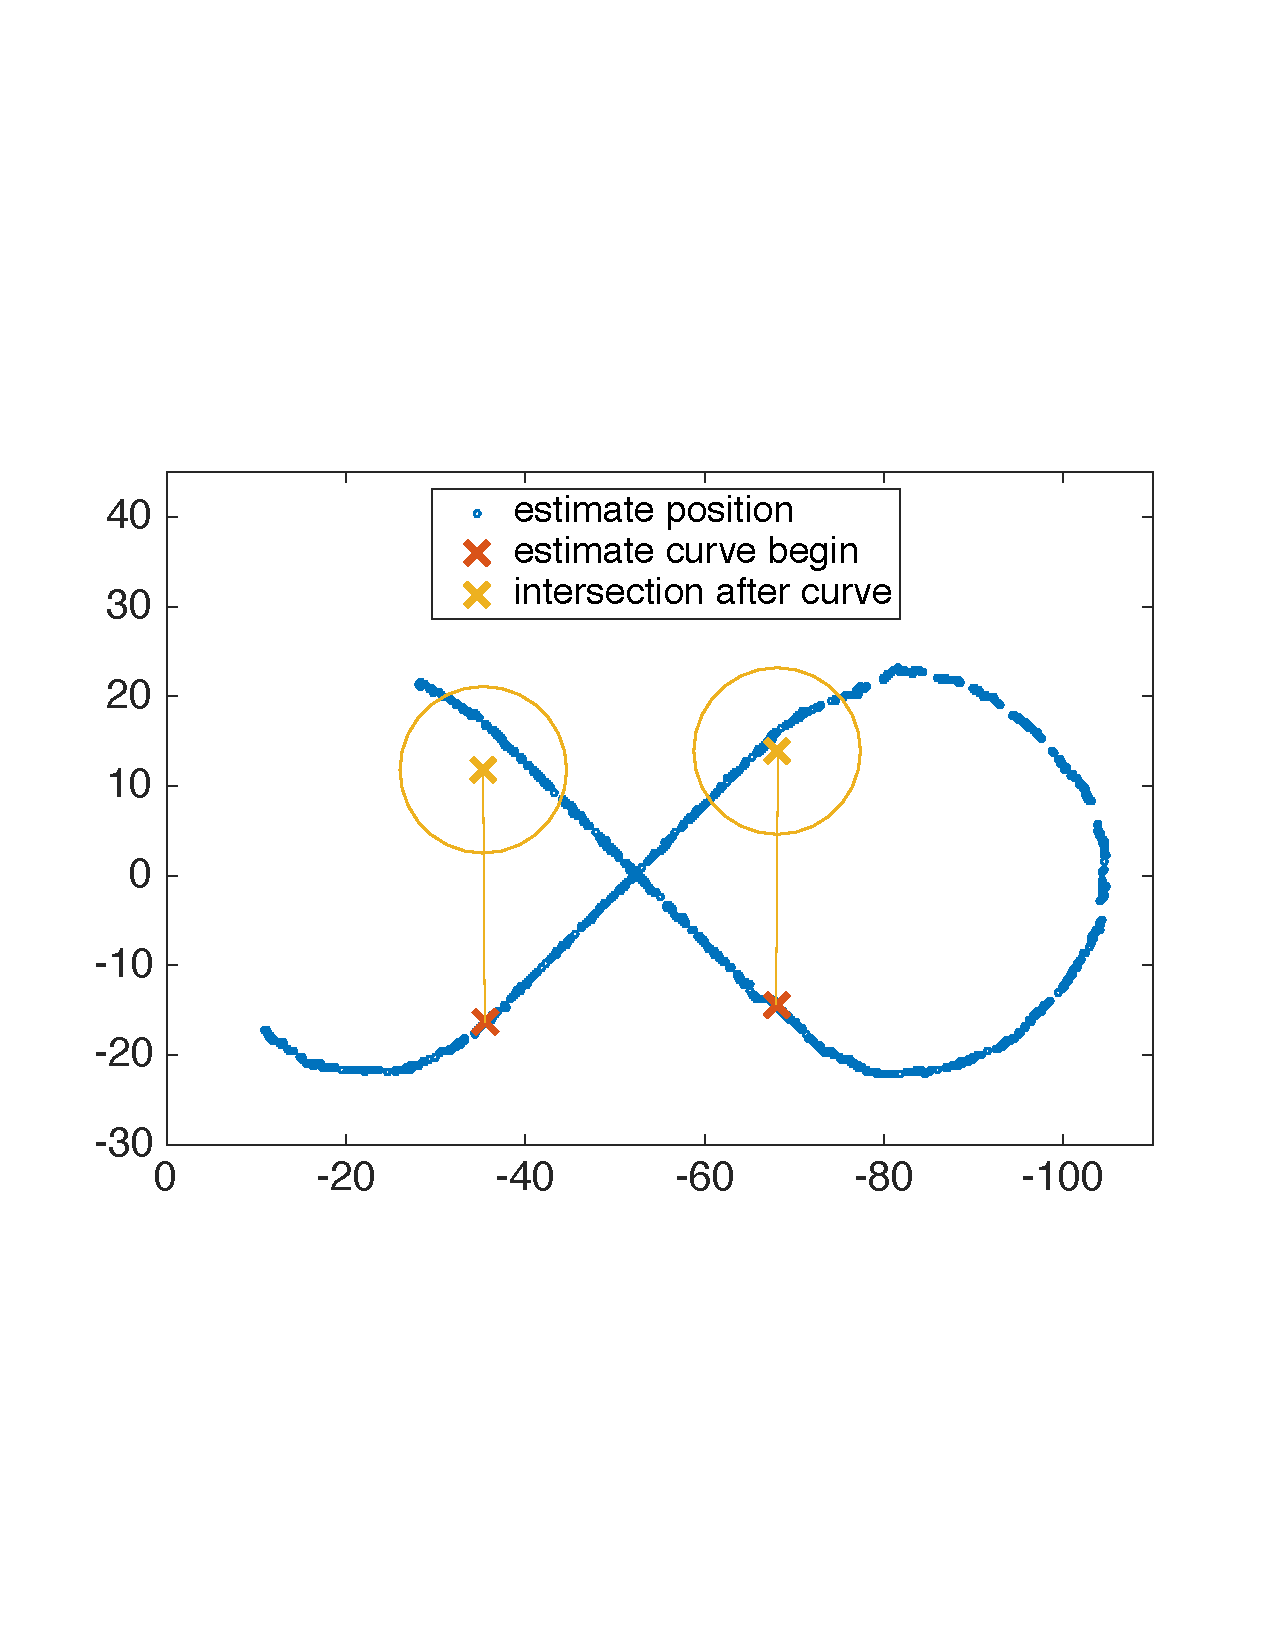
\includegraphics[width=1.0\textwidth]{img/following_platform_normal_map_intersection.pdf}
    \caption{Data from the first phase of the area exploration. Blue circles position of the base estimate. Red cross the points in which the algorithm detect a passage from a line phase to a curve. Green cross from a curve to a line. Yellow cross the position where the quadrotor should go in order to intersect the platform when is about to start a line phase.}
    \label{fig:map_intersections}
\end{figure}


\subsection{Second phase - Approaching the base}

\subsection{Second phase - Following the base}

\subsection{Second phase - Landing on the base}
